% vim: tw=0:wrap:linebreak
\documentclass[DM,toc]{lsstdoc}

\usepackage{datetime}
\usepackage{microtype}

\newcommand{\microarcsec}{$\mu$as\xspace}
\interfootnotelinepenalty=10000

\setcounter{secnumdepth}{3}

\title{Data Management Science Pipelines Design}
\author{
    J.D.~Swinbank,
    T.~Axelrod,  A.C.~Becker, J.~Becla, E.~Bellm,
    J.F.~Bosch,  H.~Chiang, D.R.~Ciardi,  A.J.~Connolly,  G.P.~Dubois-Felsmann,
    F.~Economou, M.~Fisher-Levine, M.~Graham, \v{Z}. Ivezi\'c,  M.~Juri\'c,
    T.~Jenness,  R.L.~Jones, J.~Kantor, S.~Krughoff, K-T.~Lim, R.H.~Lupton,
    F.~Mueller,  D.~Petravick, P.A.~Price,  D.J.~Reiss, D.~Shaw, C.~Slater,
    M.~Wood-Vasey, X.~Wu, P.~Yoachim,
     \emph{for the LSST Data Management}
}

\setDocRef{LDM-151}
\setDocCurator{J.D.~Swinbank}
\date{2017-07-19}

\setDocAbstract{%
The LSST Science Requirements Document (the LSST \SRD) specifies a set of data product guidelines, designed to support science goals envisioned to be enabled by the LSST observing program.
Following these guidlines, the details of these data products have been described in the LSST Data Products Definition Document (\DPDD), and captured in a formal flow-down from the \SRD via the LSST System Requirements (\LSR), Observatory System Specifications (\OSS), to the Data Management System Requirements (\DMSR).
The LSST Data Management subsystem's responsibilities include the design, implementation, deployment and execution of software pipelines necessary to generate these data products. This document describes the design of the scientific aspects of those pipelines.
}

%
%   Revision history
%
% OLDEST FIRST: VERSION, DATE, DESCRIPTION, OWNER NAME
\setDocChangeRecord{%
\addtohist{1}{2009-03-26}{Initial version as Document-7396}{Tim Axelrod et al.}
\addtohist{1.2}{2009-03-27}{Minor edits}{Tim Axelrod}
\addtohist{1.3}{2009-04-17}{General edits and updates}{Tim Axelrod}
\addtohist{1.4}{2009-05-08}{Explicit reference to multifit added to Section 6.1}{Tim Axelrod}
\addtohist{1.5}{2010-02-11}{General edits and updates; generated from SysML model}{Jeff Kantor}
\addtohist{2}{2011-08-04}{Elevated to LDM handle; general updates and edits}{Tim Axelrod}
\addtohist{3}{2013-10-07}{Updates for consistency with FDR baseline}{Mario Juric}
\addtohist{}{2017-05-08}{Major reorganization for DM replan}{Mario Juric}
\addtohist{4.0}{2017-05-19}{Approved in \href{https://jira.lsstcorp.org/browse/RFC-338}{RFC-338} and released.}{Mario Juric (approval), Tim Jenness (release)}
\addtohist{4.1}{2017-07-19}{Remove development commentary. This content was included erroneously and was not part of the approved baseline.}{Tim Jenness}
}


\begin{document}

\maketitle

\section{Preface}

The purpose of this document is to describe the design of pipelines belonging to the Applications Layer of the Large Synoptic Survey Telescope (LSST) Data Management system. These include most of the core astronomical data processing software that LSST employs.

The intended audience of this document are LSST software architects and developers. It presents the baseline architecture and algorithmic selections for core DM pipelines, developed to a degree necessary to enable planning and costing of the pipelines assuming an Agile software development framework. The document assumes the reader/developer has the required knowledge of astronomical image processing algorithms and solid understanding of the state of the art of the field, understanding of the LSST Project goals and concepts, and has read the LSST Science Requirements (\SRD) as well as the LSST Data Products Definition Document (\DPDD).

% This document should be read in conjunction with the LSST DM Applications Use Case Model (\appsUMLusecase). They are intended to be complementary, with the Use Case model capturing the detailed (inter)connections between individual pipeline components, and this document capturing the overall goals, pipeline architecture, and algorithmic choices.

Though under strict change control, this is a \textbf{\emph{living document}}. Firstly, as a consequence of the ``rolling wave'' LSST software development model, the designs presented in this document will be refined and made more detailed as particular pipeline functionality is about to be implemented. Secondly, the LSST will undergo a period of construction and commissioning lasting no less than seven years, followed by a decade of survey operations. To ensure their continued scientific adequacy, the overall designs and plans for LSST data processing pipelines will be periodically reviewed and updated.


\section{Introduction}

\subsection{LSST Data Management System}

To carry out this mission the Data Management System (DMS) performs the following major functions:

\begin{itemize}
\item Processes the incoming stream of images generated by the camera
  system during observing to produce transient alerts and to archive
  the raw images.

\item Roughly once per year, creates and archives a Data Release (``DR''),
  which is a static self-consistent collection of data products
  generated from all survey data taken from the date of survey
  initiation to the cutoff date for the Data Release. The data
  products (described in detail in the \DPDD), include measurements of 
  the properties (shapes, positions, fluxes, motions, etc.) of all detected
  objects, including those below the single visit sensitivity limit,
  astrometric and photometric calibration of the full survey object
  catalog, and limited classification of objects based on both their
  static properties and time-dependent behavior.  Deep coadded images
  of the full survey area are produced as well.

\item Periodically creates new calibration data products, such as bias
  frames and flat fields, that will be used by the other processing
  functions, as necessary to enable the creation of the data products above.

\item Makes all LSST data available through interfaces that utilize,
  to the maximum possible extent, community-based standards such as those
  being developed by the Virtual Observatory (``VO''), and facilitates user
  data analysis and the production of user-defined data products at Data
  Access Centers (``DAC'') and at external sites.
\end{itemize}

The overall architecture of the DMS is discussed in more detail in the Data Management System Design (\DMSD) document. The overall architecture of the DMS is shown in Figure~\ref{fig:DMS}.
\\

This document discusses the role of the Applications layer in the first three functions listed above (the functions involving \emph{science pipelines}).  The fourth is discussed separately in the SUI Conceptual Design Document (\SUI).

\begin{figure}
\centering
\includegraphics[angle=90,scale=0.70]{figures/DMS-Architecture.pdf}
\caption{Architecture of the Data Management System\label{fig:DMS}}
\end{figure}

\begin{figure}
%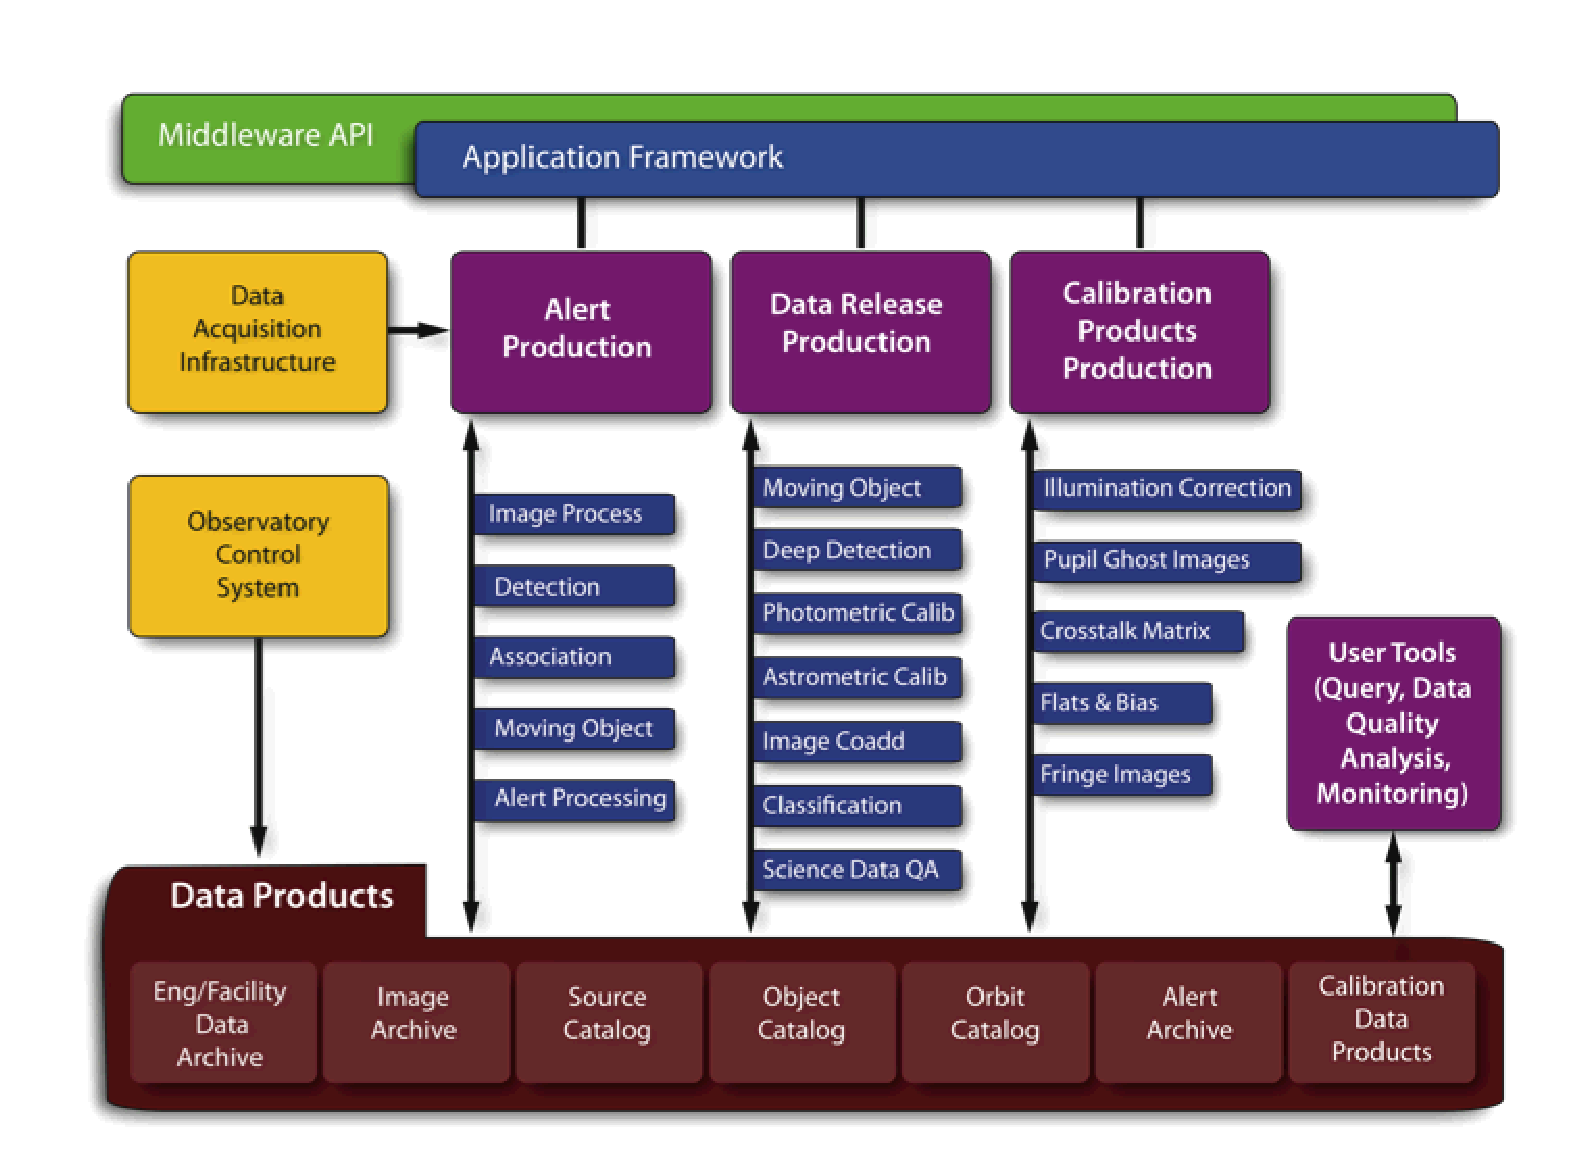
\includegraphics[angle=90,scale=0.70]{ApplicationLayerProductionsandPipelines.eps}
\centering
\includegraphics[angle=90]{figures/DataProductDelivarables.png}
\caption{Organization of LSST Data Products\label{fig:DP}}
\end{figure}

\subsection{Data Products}

The LSST data products are organized into three groups, based on their intended use and/or origin. The full description is provided in the Data Products Definition Document (\DPDD); we summarize the key properties here to provide the necessary context for the discussion to follow. 

\begin{itemize}
\item {\bf Level 1} products are intended to support timely detection and follow-up
  of time-domain events (variable and transient sources). They are generated by
  near-real-time processing the stream of data from the camera system during 
  normal observing.  Level 1 products are therefore continuously generated and / or
  updated every observing night. This process is of necessity highly
  automated, and must proceed with absolutely minimal human
  interaction.  In addition to science data products, a number of related
  Level 1 ``SDQA''\footnote{Science Data Quality Analysis} data products are generated
  to assess quality and to provide feedback to the Observatory Control System (OCS).

\item {\bf Level 2} products are generated as part of a Data Release, generally
  performed 
  yearly, with an additional data release for the first 6 months of survey data. 
  Level 2 includes data products for which extensive
  computation is required, often because they combine information from
  many exposures.  Although the steps that generate Level 2 products
  will be automated, significant human interaction may be required at
  key points to ensure the quality of the data.

\item {\bf Level 3} products are generated on any computing resources
  anywhere and then stored in an LSST Data Access Center. Often, but not
  necessarily, they will be generated by users of LSST using LSST software
  and/or hardware. LSST DM is required to facilitate the creation of
  Level 3 data products by providing suitable APIs, software components, and
  computing infrastructure, but will not by itself create any Level 3
  data products. Once created, Level 3 data products may be associated with
  Level 1 and Level 2 data products through database federation.
  Where appropriate, the LSST Project, with the agreement of the Level 3
  creators, may incorporate user-contributed Level 3 data product pipelines
  into the DMS production flow, thereby promoting them to Level 1 or 2.

\end{itemize}

\begin{note}{JFB comment:}
Should we mention intermediate data products as a category here, too?  Those will be an important part of the Pipeline descriptions that happen later in the document.
\end{note}

The organization of LSST Data Products is shown in Figure~\ref{fig:DP}.

Level 1 and Level 2 data products that have passed quality control
tests will be accessible to the public without restriction.
Additionally, the source code used to generate them will be made
available, and LSST will provide support for builds on selected
platforms.

\subsubsection{Data Units}

\begin{note}[TODO]
  This section still in outline form.
\end{note}

\begin{itemize}
  \item Source vs. Object
  \item Visit, CCD, Snap
  \item Tract, Patch
  \item Filters and object SEDs
\end{itemize}

\subsection{Science Pipelines Organization}

\begin{note}[TODO]
  This section still in outline form.  Expanded form should be short; I'm proposing we move the longer overviews that used to be in the introductions into the beginning of the sections for each Production, and shorten them to little more than a description of that Production's overview diagram.
\end{note}

\begin{itemize}
\item In sections (bla) we describe Alert Production, Calibration Product Production, and Data Release Production by decomposing them Pipelines.  Pipelines are not reusable; they occupy a specific place in a Production.
\item In section (bla) we describe the SDQA system, a set of smaller Productions as well as independent Pipelines within AP and DRP that verify the quality of the algoritms and data.
\item In section (bla) we say something with scope TBD about SUIT and enabling Level 3.
\item Pipelines are composed of reusable Algorithmic Components, which are described in section (bla).
\item Algorithmic Components rely on shared software primitives, described in section (bla).

\end{itemize}


\section{Alert Production}
\label{sec:ap}



Alert Production is run each night to product catalogs and images for sources that have varied or moved relative to a previous observation.  The data products produced by Alert production are given in  table~\ref{table:ap_data_products}.

\begin{table}
\small
\begin{tabularx}{\textwidth}{ | l | l | X | }
  \hline
  {\bf Name} & {\bf Availability} & {\bf Description} \\
  \hline
  DIASource & Stored &
  Measurements from difference imagine analysis of individual exposures. \\
  \hline
  DIAObject& Stored &
  Aggregate quantities computing by associating spatially colocated DIASources. \\
  \hline
  DIAForcedSource & Stored &
  Flux measurements on each difference image at the position of every DIAObject. \\
  \hline
  SSObject & Stored &
  Solar system objects derived by associating DIASources and inferring their orbits. \\
  \hline
  CalExp & Stored &
  Calibrated exposure images for each CCD/visit (sum of two snaps). \\
  \hline
  DiffExp & Stored &
  Difference between CalExp and PSF-matched template coadd. \\
  \hline
\end{tabularx}
\caption{Table of derived and persisted data products produced during a Alert Production.  A description of these data products can be found in the Data Products Definition Document (LSE-163).
\label{table:ap_data_products}}
\end{table}


Alert Production is designed as five separate components: single frame
processing, alert detection, alert generation, precovery photometry,
and a moving objects pipeline. The first four of these components run
as a linear pass through of the data. The moving objects pipeline is
run independently of the rest of the alert production. The flow of
information through this system is shown in figure~\ref{fig:nightly}.

\begin{figure}[th]
\begin{center}
\includegraphics[width=0.9\textwidth]{figures/Level_1_Processing_Flowchart.jpg}
\caption{\label{fig:nightly} The alert production flow of data through
  the processing pipelines (single frame processing, alert detection,
  alert generation, precovery photometry) }
\end{center}
\end{figure}

\subsection{Single Frame Processing Pipeline (\wbsSFM)}
\label{sec:apSingleFrameProcessing}

Single Frame Processing (SFM) Pipeline is responsible for reducing raw or camera corrected image data to \emph{calibrated exposures}, the detection and measurement of \Sources (using the components functionally a part of the Object Characterization Pipeline), the characterization of the point-spread-function (PSF), and the generation of an astrometric solution for an image.

\subsubsection{Baseline Design}

Single Frame Processing pipeline will be implemented as a flexible   framework where new processing steps can be added without modifying the stack code. It should be possible for this pipeline or a subset of this pipeline  to be run at the telescope facility during commissioning and operations.  

\paragraph{Input Data: Raw}

Amplifier images that the camera has corrected for crosstalk, overscan, linearity.  All images from a visit should be available to the task (including snaps). An approximate WCS is assumed to be available as metadata

\paragraph{Input Data Product: Reference}

A full-sky reference catalog of stars derived either from an external survey (e.g.\ Gaia) or from the Data Release Processing.

Flatfield calibration images for all passbands and all CCDs appropriate for the time at which the observations were undertaken

List of the positions and extents of sensor defects for all CCDs within the focal plane

Metadata for all CCDs including electronic parameters (saturation limits, readnoise, electronic footprint)

\paragraph{Output Data Product: CalExp}

A calibrated exposure (CalExp).  CalExp is an \hyperref[sec:spImagesExposure]{Exposure} object. The CalExp will contain a PSF, WCS, PhotoCalib and Background. The pixel data will include the image, mask, and variance. 

\paragraph{Output Data Product: Source}

A catalog of Sources with measured features (as described in \ref{sec:ac}). 


\paragraph{Output Data Product: Metadata}
A parameterization of the PSF for the visit, the WCS for the visit,
and associated metadata (e.g.\ photometric depth) must be made
available to the telescope Observatory Control System (OCS). It is
expected that these data will be persisted within a database that will
be queried by the OCS.


SFM pipeline functions include:
\begin{itemize}
\item Assembly of per-amplifier images to an image of the entire CCD;
\item Instrumental Signature Removal;
\item Cosmic ray rejection and snap combining;
\item Per-CCD determination of zeropoint and aperture corrections;
\item Per-CCD PSF determination;
\item Per-CCD WCS determination and astrometric registration of images;
\item Per-CCD sky background determination;
\item Source detection and measurement on single frame images
\item Generation of metadata required by the OCS
\end{itemize}

Calibrated exposure produced by the SFM pipeline must possess all information necessary for measurement of source properties by single-epoch Object Characterization algorithms.

\paragraph{Actions in case of failure:}

In the case camera data are not available due to a network outage that is longer than the data buffer at the summit the single frame processing will work on raw images (i.e.\ without the camera pixel corrections) and be run in a batch mode. 



\paragraph{Instrumental Signature Removal:}~
\label{sec:apISR}
Instrumental Signature Removal characterizes, corrects, interpolates
and flags the camera (or raw) images to generate a flat-fielded and corrected
exposure.

\paragraph{Pipeline Tasks}
\begin{itemize}
\item Mask CCD defects based on the and saturation
\item Assembly
\item Full frame corrections: Dark, Flats (includes fringing)
\item Pixel level corrections: Brighter fatter, static pixel size effects
\item Interpolation of defects and saturation
\item \hyperref[sec:artifact]{CR rejection}
\item Generate snap difference
\item Snap combination
\end{itemize}


\paragraph{PSF and background determination:}~
\label{sec:apPSFBackground}

Given exposures that have been processed through the Instrument Signature Removal, sources must be detected that will be used to determine the WCS and photometric calibration of the images. Detection and measurement of the properties of these calibration Sources requires knowlege of the PSF and background for the image which in turn requires knowledge of the sources on the image. An iterative procedure is, therefore, adopted to generate the Source catalog. 

\paragraph{Pipeline Tasks}
The procedure for PSF and background estimation and the associated
algorithmic components. Convergence criteria for the procedure is not
defined but the default procedure assumes three iterations.
\begin{itemize}
\item \hyperref[sec:acBackgroundEstimation]{Background estimation}
\item \hyperref[sec:acSourceDetection]{Source detection} to the 5$\sigma$ limit of
%\item Single CCD \hyperref[sec:acDeblending]{Deblend sources}
\item Selection of PSF candidate stars based on a signal-to-noise threshold 
  (default 50 $\sigma$) and isolated sources 
\item Single CCD \hyperref[sec:acSingleCCDPSF]{PSF determination} given the selected bright sources
%\item Single CCD \hyperref[sec:acModelSpatialPSF]{PSF spatial model}
\end{itemize}


\paragraph{Source measurement:}~
\label{sec:apSourcemeasurement}

For the Source catalog generated in \label{sec:apPSFBackground} measure the source properties using a subset of features measured in \label{sec:drpMeasureSources}. Source measurement if for all sources within the Source catalog and not just the bright subset used to calibrate the PSF. 

\paragraph{Pipeline Tasks}
We anticipate using the following plugin algorithms for \label{sec:drpMeasureSources}
\begin{itemize}
\item \hyperref[sec:acCentroidAlgorithms]{Centroids}
\item \hyperref[sec:acPixelFlags]{Pixel Flag Aggregation}
\item \hyperref[sec:acAperturePhotometry]{Aperture Photometry} (but only for one or two radii) 
\item \hyperref[sec:acPSFPhotometry]{PSF Photometry} 
\item \hyperref[sec:acStaticPointSourceModels]{Static Point Source Models}
\item  \hyperref[sec:apertureCorrection]{Aperture correction} for  detected sources
\end{itemize}

\paragraph{Photometric and Astrometric calibration:}~
Photometric and astrometric calibration entails a ``semi-blind'' cross match of a reference catalog (derived either from the DRP Objects or from an external catalog), the generation of a WCS (on the scale of a CCD or visit), and the generation of a photometric zeropoint (on the scale of a CCD).

\paragraph{Pipeline Tasks}
Photometric and astrometric calibration performed at the scale of a
single sensor (extended to the scale of a visit depending on required fidelity)
\begin{itemize}
\item CCD level \hyperref[sec:acSingleCCDReferenceMatching]{source
    association} between the DRP reference catalog and Sources from the \ref{sec:apSourcemeasurement}
\item Generation of a \hyperref[sec:acSingleCCDPhotometricFit]{photometric solution} at the level of a single CCD
\item Decomposition of the astrometric components (e.g.\ optical distortions, sensor tree-rings) for a single CCD and generation of an \hyperref[sec:acSingleCCDAstrometricFit]{astrometric fit} at the level of a single CCD
\item Persistence of the astrometric, PSF, and photometric solutions so that the OCS can incorporate it into their telemetry
\end{itemize}

Given the number of stars available on a CCD or the complexity of the astrometric solutions for the LSST it may be necessary that the astrometric and photometric solutions must be performed at the level of a visit and not a CCD.  For these cases the operations will be \hyperref[sec:acSingleVisitReferenceMatching]{single visit matching},   \hyperref[sec:acSingleCCDPhotometricFit]{single visit photometric solutions}, \hyperref[sec:acSingleVisitAstrometricFit]{single visit astrometric fits}.

Astrometric and photometric performance within crowded fields will require that the order of the WCS should depend on the number of calibration Sources that are available.

\clearpage

\subsection{Alert Detection (\wbsDiffim)}
\label{sec:apAlertDetection}

\noindent 
{\bf Input Data:}\\
\begin{itemize}
\item Butler access to Coadd images from DRP that overlap spatially
  with CalExp images 
\item Access to DIAObjects that overlap spatially with CalExp images 
\item Access to Objects that overlap spatially  with CalExp images 
\item Access to SSObjects whose ephemerides overlap spatially  with CalExp images 
\item Internal reference catalog for CalExp from DRP 
\item PSF \hyperref[sec:apSingleFrameProcessing]{measured} from the
  science image.
\item Data structures for the real-bogus classifier
\end{itemize}


{\bf Output Data}\\
\begin{itemize}
\item DIAimage persisted
\item DIASources persisted
\item DIAObjects persisted
\item DIA forced photometry persisted
\end{itemize}

{\bf Actions in case of failure:}\\
{\bf Alternative procedures:}\\
\begin{itemize}
\item Butler access to CalExp images from DRP that overlap spatially
  with current CalExp image  for template generation
\end{itemize}
\subsubsection{Key Requirements}

The alert detection pipeline shall difference a visit image against a deeper template, and detect and characterize sources in the difference image in the time required to achieve the 60 second design goal for Level 1 alert processing (current timing allocation: 24 seconds). The algorithms employed by the pipeline shall result in purity and completeness of the sample as required by the \DMSR\@. Image differencing shall perform as well in crowded as in uncrowded fields.

\subsubsection{Baseline Design}
\label{sec:diffimDesign}

\paragraph{Template Generation}~

By either querying for Coadd Images that spatially overlap with a
given CalExp or for a DCR differential chromatic refraction corrected
template (see \hyperref[sec:acRetrieveTemplate]{Retrieve Diffim
  Template}) template image.

\noindent
{\bf Subtasks:}
\begin{itemize}
\item Query for Coadd images that are within a given time interval
  (default 2 years) of the current sensor image, and are within
  allowable airmass limits (default XXX). seexs
  \hyperref[sec:acRetrieveTemplate]{template retrieval}
\item An alternate approach will be to return an interpolated,
  DCR-corrected template based on a model of the effect of DCR (see
  \hyperref[sec:acDCRTemplates]{ DCR template generation}). The
  direction of the DCR correction will be aligned with the 
  ``parallactic angle''.
  \end{itemize}

\paragraph{Image differencing}~

Model the matching kernel and its spatial variation using a regression
approach and a \hyperref[sec:acImageSubtraction]{set of basis functions}

\noindent
{\bf Subtasks:}
\begin{itemize}
\item Match \hyperref[sec:apSourcemeasurement]{DRP} sources and
  sources from \hyperref[sec:apSingleFrameProcessing]{SFP}
\item Determine a relative astrometric solution
\item Warp the template and measurements to the science image frame
\item Determine the appropriate PSF matching sources
\item Decorrelate the science image with an estimate of the science PSF (pre-convolution) 
\item Compute the PSF matching kernel and spatial model using
  \hyperref[sec:acDiffImDecorrelation]{ZOGY} approach
\item Difference the science and template images
\item Apply a correction for correlated noise
\item Difference image \hyperref[sec:acSourceDetection]{source
    detection} to generate DIASources
\item Difference image  \hyperref[sec:acMeasurement]{source
    measurement}: \hyperref[sec:acDipoleModels]{dipole fit}, \hyperref[sec:acTrailedPointSourceModels]{trailed source} measurement
\item Measure flux on snap difference for all DIASources
\end{itemize}

\paragraph{Real-Bogus classification}~

Initial classification step to identify false positives in the image
difference sources. Training of the classifier will be undertaken
outside of the nightly processing and will utilize a training sample
of real variable sources and artifacts based on labelled data. Labels
will be derived from simulated data and visually classified sources.

\noindent
{\bf Subtasks:}
\begin{itemize}
\item The data structures for the real-bogus machine learning
  algorithm(s) will be loaded
\item A random forest or other probabilistic classification algorithm will be
  applied to the DIASources
\item Update the DIASources with the probabilistic classification 
\item Prune the DIASource list based on classifier results
\end{itemize}

\paragraph{Source Association}~

{\bf Input Data:}\\
\begin{itemize}
\item Access to DIAObjects and that overlap spatially with CalExp images
\item Access to Objects that overlap spatially  with CalExp images
\item Access to SSObjects whose \hyperref[sec:acEphemerisCalculation]{ephemerides} overlap spatially with CalExp images
\item Internal reference catalog for CalExp from DRP
\item PSF \hyperref[sec:apSingleFrameProcessing]{measured} from the
  science image
\item Data structures for the real-bogus classifier
\end{itemize}


{\bf Output Data}\\
\begin{itemize}
\item DIAimage persisted
\item DIASources persisted
\item DIAObjects persisted
\item DIA forced photometry persisted
\end{itemize}
\noindent
{\bf Subtasks:}
\begin{itemize}
\item Given the time of an observation and the motion of the sources,
  propagate positions of all sources (SSObjects and DIASources).
\item Using the WCS determine the sensor coordinates for all
  DIAObjects in the catalog
\item Match all DIASources to all DIAObject catalog positions using a probabilistic \hyperref[sec:acDIAObjectGeneration]{matching algorithm}
\item Update associated DIAObjects with aggregate quantities
  e.g. position and flux (in a 30 day rolling wind)
\item Perform forced photometry of all DIAObjects that intersect with
  the frame.
\end{itemize}


\subsubsection{Prototype Implementation}

The prototype code is available at \url{https://github.com/lsst/ip_diffim}. The current prototype, while functional, will require a partial redesign to be transfered to construction to address performance and extensibility concerns.

\clearpage

\subsection{Alert Generation Pipeline (\wbsAP)}

\subsubsection{Key Requirements}

Alert Generation Pipeline shall take the newly discovered \DIASources and all associated metadata as described
in the \DPDD, and deliver alert packets in \VOEvent format to a variety of endpoints via standard IVOA protocols (eg., VOEvent Transport Protocol; VTP\@).

To directly serve the end-users, the Alert Generation Pipeline shall provide a basic, limited capacity, alert filtering service. This service will run at the LSST U.S. Archive Center (at NCSA). It will let astronomers create simple filters that limit what alerts, and what fields from those alerts, are ultimately forwarded to them. These \emph{user defined filters} will be possible to specify using an SQL-like declarative language, or short snippets of (likely Python) code.

Since there is a need to keep both the alert database and the brokers consistent, there is a big win if both the database and the brokers read from the same fault tolerant intermediate persistence format.  A redundant, cluster based, strongly ordered, message system like Kafka (http://kafka.apache.org) is a very attractive option as the intermediate persistence.  It is very similar in concept to persisting to some well known file format with the addition of reduntant storage, configurable expiration time of messages, and strict ordering so database catch-up is trivial.  It is also scalable.

\subsubsection{Baseline Design}

{\bf Input Data:}\\
\begin{itemize}
\item Access to DIAObjects that overlap spatially with CalExp images
\item Access to Template image that overlap spatially with CalExp images
\end{itemize}


{\bf Output Data}\\
\begin{itemize}
\item DIA event table persisted
\item VOEvents
\end{itemize}

\paragraph{Alert generation}~

\noindent
{\bf Subtasks:}
\begin{itemize}
\item Generate postage stamps for all DIASources: direct image and difference image
\item Push alert records to alert persistence
\item Alert database ingestion client reads all new alerts and persists them permanently in the alert database
\end{itemize}

\paragraph{Alert Distribution: To community brokers}
\noindent
{\bf Subtasks:}
\begin{itemize}
\item For each visit read all new alert records from the alert persistence
\item Package each message as a properly formatted VOEvent
\item Bundle VOEvents using a pre-negotiated format
\item Transmit bundled VOEvents to community broker endpoints
\end{itemize}

\paragraph{Alert Distribution: Minimal brokers}
\noindent
Each minimal broker will have some subset of users.  The following is for a single broker.
{\bf Subtasks:}
\begin{itemize}
\item Read new alert records from the alert persistence in order
\item Filter event records for relevance (WHERE)
\item Filter event columns for content (SELECT)
\item Package event as a valid VOEvent
\item Publish the VOEvent to the appropriate endpoint (potentially another messaging queue so clients can access asynchronosly)
\end{itemize}

\paragraph{Forced Photometry on all DIAObjects}~

\noindent
{\bf Subtasks:}
\begin{itemize}
\item Compute forced photometry on all DIAObjects in the field.  This
  does not end up in the alerts.
\item Update the DIA Object forced photometry tables
\end{itemize}

\subsubsection{Prototype Implementation}

\clearpage

\subsection{Precovery Photometry Pipeline}

\noindent
{\bf Input Data:}\\
\begin{itemize}
\item Butler access to DIA images within finite time interval (default 
  30 days) 
\item Butler access to DIAobjects detected from the previous night 
  with no associations 
\end{itemize}
{\bf Output Data}\\
\begin{itemize}
\item Updated and persisted forced photometry tables for all newly
  detected DIAobjects
\end{itemize}

\subsubsection{Key Requirements}

Within 24 hrs.

\paragraph{Precovery of new DIAObjects}~

\noindent
{\bf Subtasks:}
\begin{itemize}
\item Force photometer in difference images for all new DIAObjects for the past 30 days.
\end{itemize}
\clearpage

\subsection{Moving Object Pipeline (\wbsMOPS)}

\subsubsection{Key Requirements}

The Moving Object Pipeline is responsible for generating and managing the Solar System\footnote{Also sometimes referred to as `Moving Object'} data products. These are Solar System objects with associated Keplerian orbits, errors, and detected \DIASources. Quantitatively, it shall be capable of detecting 95\% of all Solar System objects that meet the findability criteria as defined in the \OSS\@. 

\subsubsection{Baseline Design}
{\bf Input Data}\\
\begin{itemize}
\item 'Orphan' DIASources from the last night of observing.  This means DIASources that are not associated with a DIAObject.  DIASources associated with an SSObject in the night are still passed through the MOPS machinery
\item DIAObject database
\item SSObject database
\item Exposure metadata database
\end{itemize}
{\bf Output Data}\\
\begin{itemize}
\item Updated SSObject databaase
\item Updated DIASource database
\end{itemize}
{\bf Anscillary Products}\\
\begin{itemize}
\item Tracklet database
\item Track database
\item Intermediate orbit prediction database
\end{itemize}
{\bf Actions in case of failure}\\
{\bf Alternative procedures}\\

{\bf Subtasks:}
\begin{itemize}
\item Feed all input orphan DIASources to \hyperref[sec:acMakeTracklets][makeTracklets].
\item Run \hyperref[sec:acAttributionAndPrecovery]{attribution and precovery} on with just the tracklets and DIASources from the previous night.  This culls any tracklets or DIASources that obviously belong to an existing SSObject from the rest of the processing.
\item Compute new \hyperref[sec:acOrbitFitting]{orbits} and \hyperref[sec:acOrbitMerging]{merge orbits}.
\item Run \hyperref[sec:acAttributionAndPrecovery]{attribution and precovery} on with full survey of tracklets and DIASources but only running over new SSObjects.
\item \hyperref[sec:acOrbitMerging]{Merge Orbits}.
\end{itemize}

\subsubsection{Prototype Implementation}

Prototype MOPS codes are available at
\url{https://github.com/lsst/mops_daymops} and
\url{https://github.com/lsst/mops_nightmops}. We expect it will be
possible to transfer a significant fraction of the existing code into
Construction. Current DayMOPS prototype already performs within the
computational envelope envisioned for LSST Operations, though it does
not yet reach the required completeness requirement.



\section{Calibration Products Production}
\label{sec:cpp}

\subsection{Calibration Products Pipeline (\wbsCPP)}

\subsubsection{Key Requirements}

The work performed in this WBS serves two complementary roles:

\begin{itemize}
  \item{It will enable the production of calibration data products as required by the Level 2 Photometric Calibration Plan (\NewPCP{}) and other planning documents \cite{Lupton15}\footnote{Resolving contradictions between these documents is out of scope here.}. This includes both characterization of the sensitivity of the LSST system (optics, filters and detector) and the transmissivity of the atmosphere.}
  \item{It will characterize of detector anomalies in such a way that they can be corrected either by the instrument signature removal routines in the Single Frame Processing Pipeline (\wbsSFM) or, if appropriate, elsewhere in the system;}
  \item{It will manage and provide a catalog of optical ghosts and glints to other parts of the system upon demand.}
\end{itemize}

\subsubsection{Baseline Design}

\paragraph{Instrumental sensitivity}

We expect laboratory measurements of the filter profiles. We further baseline the development of a procedure for measuring the filter response at 1\,nm resolution using the approach described in \cite{Lupton15}.

We baseline the following procedure for creating flat fields:

\begin{enumerate}
  \item{Record bias/dark frames;}
  \item{Use ``monochromatic'' (1\,nm) flat field screen flats with no filter in the beam to measure the per-pixel sensitivity;}
  \item{Use a collimated beam projector (CBP) to measure the quantum efficiency (QE) at a set of points in the focal plane, dithering those points to tie them together;}
  \item{Combine the screen and CBP data to determine the broad band (10--100\,nm) QE of all pixels;}
  \item{Fold in the filter response to determine the 1\,nm resolution effective QE of all pixels.}
\end{enumerate}

This WBS is responsible for the development of the data analysis algorithms and software required and the ultimate delivery of the flat fields. Development and commissioning of the CBP itself, together with any other infrastructure required to perform the above procedure, lies outwith Data Management (see 04C.08 \emph{Calibration System}).

\paragraph{Atmospheric transmissivity}

Measurements from the auxiliary instrumentation---to include the 1.2\,m ``Calypso'' telescope, a bore-sight mounted radiometer and satellite-based measurement of atmospheric parameters such as pressure and ozone---will be used to determine the atmospheric absorption along the line of sight to standard stars. The atmospheric transmission will be decomposed into a set of basis functions and interpolated in space in time to any position in the LSST focal plane.

This WBS will develop a pipeline for accurate spectrophotometric measurement of stars with the auxiliary telescope. We expect to repurpose and build upon publicly available code e.g.\ from the PFS\footnote{Subaru's Prime Focus Spectrograph; \url{http://sumire.ipmu.jp/pfs/}.} project for this purpose.

This WBS will construct the atmospheric model, which may be based either on \textsc{modtran} (as per \NewPCP{}) or a PCA-like decomposition of the data (suggested by \cite{Lupton15}).

This WBS will define and develop the routine for fitting the atmospheric model to each exposure from the calibration telescope and providing estimates of the atmospheric transmission at any point in the focal plane upon request.

\paragraph{Detector effects}

An initial cross-talk correction matrix will be determined by laboratory measurements on the Camera Calibration Optical Bench (CCOB). However, to account for possibile instabilities, this WBS will develop an on-telescope method. We baseline this as being based on measurement with the CBP, but we note the alternative approach based on cosmic rays adopted by HSC \cite{Furusawa14}.

Multiple reflections between the layers of the CCD give rise to spatial variability with fine scale structure in images which may vary with time \cite[\S2.5.1]{Lupton15}. These can be characterized by white light flat-fields. Preliminary analysis indicates that these effects may be insignificant in LSST \cite{Rasmussen15}; however, the baseline calls for a a routine developed in this WBS to analyse the flat field data and generate fringe frames on demand. This requirement may be relaxed if further analysis (outside the scope of thie WBS) demonstrates it to be unnecessary.


This WBS will develop algorithms to characterize and mitigate anomalies due to the nature of the camera's CCDs.

\begin{note}
There's a complex inter-WBS situation here: the actual mitigation of CCD anomalies will generally be performed in SFM (\wbsSFM{}), based on products provided by this WBS which, in turn, may rely on laboratory based research which is broadly outside the scope of DM\@. We baseline the work required to develop the corrective algorithms here. We consider moving it to \wbsSFM{} in future.
\end{note}

The effects we anticipate include:

\begin{itemize}
  \item{QE variation between pixels;}
  \item{Static non-uniform pixel sizes (e.g.\ ``tree rings'' \cite{Stubbs14});}
  \item{Dynamic electric fields (e.g.\ ``brighter-fatter'' \cite{Antilogus14});}
  \item{Time dependent effects in the camera (e.g.\ hot pixels, changing cross-talk coefficients);}
  \item{Charge transfer (in)efficiency (CTE).}
\end{itemize}

Laboratory work required to understand these effects is outwith the scope of this WBS\@. In some cases, this work may establish that the impact of the effect may be neglected in LSST\@. The baseline plan addresses these issues through the following steps:

\begin{itemize}
  \item{Separate QE from pixel size variations\footnote{Refer to work by Rudman.} and model both as a function of position (and possibly time);}
  \item{Learn how to account for pixel size variation over the scale of objects (e.g.\ by redistributing charge);}
  \item{Develop a correction for the brighter-fatter effect and develop models for any features which cannot be removed;}
  \item{Handle edge/bloom using masking or charge redistribution;}
  \item{Track defects (hot pixels);}
  \item{Handle CTE, including when interpolating over bleed trails.}
\end{itemize}

\paragraph{Ghost catalog}

The Calibration Products Pipeline must provide a catalog of optical ghosts and glints which is available for use in other parts of the system. Detailed characterization of ghosts in the LSST system will only be possible when the system is operational. Our baseline design therefore calls for this system to be prototyped using data from precursor instrumentation; we note that ghosts in e.g. HSC are well known and more significant than are expected in LSST.

\begin{note}
It is not currently clear where the responsibility for characterizing ghosts and glints in the system lies. We assume it is outwith this WBS.
\end{note}

\subsubsection{Constituent Use Cases and Diagrams}

Produce Master Fringe Exposures; Produce Master Bias Exposure; Produce Master Dark Exposure; Calculate System Bandpasses; Calculate Telescope Bandpasses; Construct Defect Map; Produce Crosstalk Correction Matrix; Produce Optical Ghost Catalog; Produce Master Pupil Ghost Exposure; Determine CCOB-derived Illumination Correction; Determine Optical Model-derived Illumination Correction; Create Master Flat-Spectrum Flat; Determine Star Raster Photometry-derived Illumination Correction; Create Master Illumination Correction; Determine Self-calibration Correction-Derived Illumination Correction; Correct Monochromatic Flats; Reduce Spectrum Exposure; Prepare Nightly Flat Exposures;

\subsubsection{Prototype Implementation}

While parts of the Calibration Products Pipeline have been prototyped by the LSST Calibration Group (see the \NewPCP for discussion), these have not been written using LSST Data Management software framework or coding standards. We therefore expect to transfer the know-how, and rewrite the implementation.

\clearpage

\subsection{Photometric Calibration Pipeline (\wbsPhotoCal)}

\subsubsection{Key Requirements}

The Photometric Calibration Pipeline is required to internally calibrate the relative photometric zero-points of every observation, enabling the Level 2 catalogs to reach the required SRD precision.

\subsubsection{Baseline Design}

The adopted baseline algorithm is a variant of ``ubercal'' \cite{Padmanabhan08, Schlafly12}. This baseline is described in detail in the Photometric Self Calibration Design and Prototype Document (\UCAL).

\subsubsection{Constituent Use Cases and Diagrams}

Perform Global Photometric Calibration;

\subsubsection{Prototype Implementation}

Photometric Calibration Pipeline has been fully prototyped by the LSST Calibration Group to the required level of accuracy and performance (see the \UCAL document for discussion). % RHL really?  I thought that they wrote a small-scale toy version.  But I may be totally out of date.
\\

As the prototype has not been written using LSST Data Management software framework or coding standards, we assume a non-negligible refactoring and coding effort will be needed to convert it to production code in LSST Construction.

\clearpage

\subsection{Astrometric Calibration Pipeline (\wbsAstroCal)}

\subsubsection{Key Requirements}

The Astrometric Calibration Pipeline is required to calibrate the relative and absolute astrometry of the LSST survey, enabling the Level 2 catalogs to reach the required SRD precision.

\subsubsection{Baseline Design}

Algorithms developed for the Photometric Calibration Pipeline (\wbsPhotoCal) will be repurposed for astrometric calibration by changing the relevant functions to minimize. This pipeline will further be aided by WCS and local astrometric registration modules developed as a component of the Single Frame Processing pipeline (\wbsSFM).
\\

Gaia standard stars will be used to fix the global astrometric system. It is likely that the existence of Gaia catalogs may make a separate Astrometric Calibration Pipeline unnecessary.

\subsubsection{Constituent Use Cases and Diagrams}

Perform Global Astrometric Calibration;

\subsubsection{Prototype Implementation}

The Astrometric Calibration Pipeline has been partially prototyped by the LSST Calibration Group, but outside of LSST Data Management software framework. We expect to transfer the know-how, and rewrite the implementation.

\section{Data Release Production}
\label{sec:drp}

\begin{figure}
\centering
\includegraphics[width=\textwidth]{figures/drp_summary.png}
\caption{Summary of the Data Release Production processing flow.  Processing is split into multiple pipelines, which are conceptually organized into the groups discussed in sections~\ref{sec:drp_imchar_and_jointcal}-\ref{sec:drp_postprocessing}.
\label{fig:drp_summary}}
\end{figure}

\begin{note}[TODO]
  Update figure to reflect changes to sections in text.
\end{note}

A Data Release Production is run every year (twice in the first year of operations) to produce a set of catalog and image data products derived from all observations from the beginning of the survey to the point the production began.  This includes running a variant of the difference image analysis run in Alert Production, in addition to direct analysis of individual exposures and coadded images.  The data products produced by a Data Release Production are summarized in table~\ref{table:drp_data_products}.


\begin{table}
\small
\begin{tabularx}{\textwidth}{ | l | l | X | }
  \hline
  {\bf Name} & {\bf Availability} & {\bf Description} \\
  \hline
  Source & Stored &
  Measurements from direct analysis of individual exposures. \\
  \hline
  DIASource & Stored &
  Measurements from difference imagine analysis of individual exposures. \\
  \hline
  Object & Stored &
  Measurements for a single astrophysical object, derived from all available information, including coadd measurements, simultaneous multi-epoch fitting, and forced photometry.  Does not include solar system objects. \\
  \hline
  DIAObject& Stored &
  Aggregate quantities computing by associating spatially colocated DIASources. \\
  \hline
  ForcedSource & Stored &
  Flux measurements on each direct and difference image at the position of every Object. \\
  \hline
  SSObject & Stored &
  Solar system objects derived by associating DIASources and inferring their orbits. \\
  \hline
  CalExp & Regenerated &
  Calibrated exposure images for each CCD/visit (sum of two snaps). \\
  \hline
  DiffExp & Regenerated &
  Difference between CalExp and PSF-matched template coadd. \\
  \hline
  DeepCoadd & Stored &
  Coadd image with a reasonable combination of depth and resolution. \\
  \hline
  EpochRangeCoadd & Renegerated &
  Coadd image that cover only a limited range of epochs. \\
  \hline
  BestSeeingCoadd & Regenerated &
  Coadd image built from only the best-seeing images. \\
  \hline
  PSFMatchedCoadd & Regenerated &
  Coadd image with a constant, predetermined PSF. \\
  \hline
\end{tabularx}
\caption{Table of public data products produced during a Data Release Production.  A full description of these data products can be found in the Data Products Definition Document (LSE-163).
\label{table:drp_data_products}}
\end{table}

From a conceptual standpoint, data release production can be split into five groups of pipelines, executed in approximately the following order:
\begin{enumerate}
\item We characterize and calibrate each exposure, estimating point-spread functions, background models, and astrometric and photometric calibration solutions.  This iterates between processing individual exposures independently and jointly fitting catalogs derived from multiple overlapping exposures.  These steps are described more fully in section~\ref{sec:drp_imchar_and_jointcal}.
\item We alternately combine images and subtract them, using differences to find artifacts and time-variable sources while building coadds that produce a deeper view of the static sky.  Coaddition and difference imaging is described in section~\ref{sec:drp_coaddition_and_diffim}.
\item After all image processing is complete, we run additional catalog-only pipelines to fill in additional object properties.  Unlike previous stages, this postprocessing is not localized on the sky, as it may use statistics computed from the full data release to improve our characterization of individual objects.  Postprocessing pipelines are described in section~\ref{sec:drp_postprocessing}.
\end{enumerate}
This conceptual ordering is an oversimplification of the actual processing flow, however; as shown in Figure~\ref{fig:drp_summary}, pipeline groups are actually interleaved.

Each pipeline in this the diagram represents a particular piece of code excuted in parallel on a specific unit of data, but pipelines may contain additional (and more complex) parallelization to further subdivide that data unit.  The processing flow also includes the possibility of iteration between pipelines, indicated by cycles in the diagram.  The number of iterations in each cycle will be determined (via tests on smaller productions) before the start of the production, allowing us to remove these cycles simply by duplicating some pipelines a fixed number of times.  The final data release production processing can thus be described as a directed acyclic graph (DAG) to be executed by the orchestration middleware, with pipelines as edges and (intermediate) data products as vertices.  Most of the graph will be generated by applications code before the production begins, using a format and/or API defined by the orchestration middleware.  Howver, some parts of the graph must be generated on-the-fly; this will be discussed further in section~\ref{sec:drpMultiFit}.


\subsection{Image Characterization and Calibration}
\label{sec:drp_imchar_and_jointcal}

\begin{note}[ImChar/JointCal Diagram]
Extract ImChar/JointCal pipelines from ``DRP Top-Level Overview'' on confluence and expand detail to show data flow and ordering of ``Task/Process'' boxes.
\end{note}

The first steps in a Data Release Production characterize the properties of individual exposures, by iterating between pixel-level processing of individual visits (``ImChar'', or ``Image Characterization'' steps) and joint fitting of all catalogs overlapping a tract (``JointCal'', or ``Joint Calibration'' steps).  All ImChar steps involve fitting the PSF model and measuring Sources (gradually improving these as we iterate), while JointCal steps fit for new astrometric (WCS) and photometric solutions while building new reference catalogs for the ImChar steps.  Iteration is necessary for a few reasons:
\begin{itemize}
\item The PSF and WCS must have a consistent definition of object centroids.  Celestial positions from a reference catalog are transformed via the WCS to set the positions of stars used to build the PSF model, but the PSF model is then used to measure debiased centroids that feed the WCS fitting.
\item The later stages of photometric calibration and PSF modeling require secure star selection and colors to infer their SEDs.  Magnitude and morphological measurements from ImChar stages are aggregated the reference catalog in the subsequent JointCal stage, allowing these colors and classifications to be used for PSF modeling in the following ImChar stage.
\end{itemize}

The ImChar and JointCal iteration is itself interleaved with background matching and difference imaging, as described in section~\ref{sec:drp_coaddition_and_diffim}.  This allows the better backgrounds and masks to be defined by comparisons between images before the final Source measurements, image characterizations, and calibrations.

Each ImChar pipeline runs on a single visit, and each JointCal pipeline runs simultaneously on all visits within a single tract, allowing tracts to be run entirely independently.

The final output data products of the ImChar/JointCal iteration are the Source table and most of the CalExp (calibrated exposure) images.  CalExp is an \hyperref[sec:spImagesExposure]{Exposure}, and hence has Image, Mask, Variance, Background, PSF, WCS, and PhotoCalib components that we will track separately.

\subsubsection{BootstrapImChar}
\label{sec:drpBootstrapImChar}

The BootstrapImChar pipeline is the first thing run on each science exposure in a data release.  It has the difficult task of bootstrapping multiple quantities (PSF, WCS, photometric calibration, background model, etc.) that each normally require all of the others to be specified when one is fit.  As a result, while the algorithmic components to be run in this pipeline are generally clear, their ordering and specific requirements are not; algorithms that are run early will have a harder task than algorithms that are run later, and some iteration will almost certainly be necessary.

A plausible (but by no means certain) high-level algorithm for this pipeline is given below in pseudocode.  Highlighted terms are described in more detail below the pseudocode block.

\lstset{
    language=Python,
    basicstyle=\scriptsize\ttfamily,
    keywordstyle=\bfseries,
    commentstyle=\color{darkgray},
    escapeinside={\%}{\%},
}

% Define a local macro that lets us refer to sections of the text
% more easily (will undefine at the end of this section).
\newcommand{\hr}[1]{\hyperref[sec:drpBootstrapImChar_#1]{#1}}

\begin{lstlisting}
def BootstrapImChar(%\hr{raw}%, %\hr{reference}%):
    # Some data products components are visit-wide and some are per-CCD;
    # these imaginary data types lets us deal with both.
    # VisitExposure also has components; most are self-explanatory, and
    # {mi} == {image,mask,variance} (for "MaskedImage").
    calexp = VisitExposure()
    sources = VisitCatalog()
    snaps = VisitMaskedImageList()  # holds both snaps, but only {image,mask,variance}
    parallel for ccd in ALL_SENSORS:
        snaps[ccd] = [%\hr{RunISR}%(raw[ccd]) for snap in SNAP_NUMBERS]
        snaps[ccd].mask = %\hr{SubtractSnaps}%(snaps[ccd])
        calexp[ccd].mi = %\hr{CombineSnaps}%(snaps[ccd])
    calexp.psf = %\hr{FitWavefront}%(calexp[WAVEFRONT_SENSORS].mi)
    calexp.{image,mask,variance,background}
        = %\hr{SubtractBackground}%(calexp.mi)
    parallel for ccd in ALL_SENSORS:
        sources[ccd] = %\hr{DetectSources}%(calexp.{mi,psf})
    sources[ccd] = %\hr{DeblendSources}%(sources[ccd], calexp.{mi,psf})
    sources[ccd] = %\hr{MeasureSources}%(sources[ccd], calexp.{mi,psf})
    matches = %\hr{MatchSemiBlind}%(sources, reference)
    while not converged:
        %\hr{SelectStars}%(matches, exposures)
        calexp.wcs = %\hr{FitWCS}%(matches, sources, reference)
        calexp.psf = %\hr{FitPSF}%(matches, sources, calexp.{mi,wcs})
        %\hr{WriteDiagnostics}%(snaps, calexp, sources)
        parallel for ccd in ALL_SENSORS:
            snaps[ccd] = %\hr{SubtractSnaps}%(snaps[ccd], calexp[ccd].psf)
            calexp[ccd].mi = %\hr{CombineSnaps}%(snaps[ccd])
            calexp[ccd].mi = %\hr{SubtractStars}%(calexp[ccd].{mi,psf}, sources[ccd])
        calexp.{mi,background} = %\hr{SubtractBackground}%(calexp.mi)
        parallel for ccd in ALL_SENSORS:
            sources[ccd] = %\hr{DetectSources}%(calexp.{mi,psf})
            calexp[ccd].mi, sources[ccd] =
                %\hr{ReinsertStars}%(calexp[ccd].{mi,psf}, sources[ccd])
            sources[ccd] = %\hr{DeblendSources}%(sources[ccd], calexp.{mi,psf})
            sources[ccd] = %\hr{MeasureSources}%(sources[ccd], calexp.{mi,psf})
        matches = %\hr{MatchNonBlind}%(sources, reference)
    calexp.psf.apcorr = %\hr{FitApCorr}%(matches, sources)
    parallel for ccd in SCIENCE_SENSORS:
        sources[ccd] = %\hr{ApplyApCorr}%(sources[ccd], calexp.psf)
    return calexp, sources
\end{lstlisting}

\paragraph{Input Data Product: Raw}
\label{sec:drpBootstrapImChar_raw}

Raw amplifier images from science and wavefront CCDs, spread across one or more snaps.  Needed telescope telemetry (seeing estimate, approximate pointing) is assumed to be included in the raw image metadata.

\paragraph{Input Data Product: Reference}
\label{sec:drpBootstrapImChar_reference}

A full-sky catalog of reference stars derived from both external (e.g. Gaia) and LSST data.

The \hyperref[sec:drpStandardJointCal]{StandardJointCal} pipeline will later define a deeper reference catalog derived from this one and the new data being processed, but the origin and depth of the initial reference catalog is largely TBD.  It will almost certainly include Gaia stars, but it may also include data from other telescopes, LSST special programs, LSST commissioning observations, and/or the last LSST data release.  Decisions will require some combination of negotation with the LSST commissioning team, specification of the special programs, quality analysis and experimentation with the Gaia catalog, and policy decisions from DM leadership on the degree to which data releases are required to be independent.  Depending on the choices selected, it could also require a major separate processing effort using modified versions of the data release production pipelines.

\paragraph{Output Data Product: Source}
\label{sec:drpBootstrapImChar_sources}

A preliminary version of the Source table.  This could contain all of the columns in the DPDD Source schema if the \hr{MeasureSources} is appropriately configured, but some of these columns are likely unnecessary in its role as an intermediate data product that feeds \hyperref[sec:drpStandardJointCal]{StandardJointCal}, and it is likely that other non-DPDD columns will be present for that role.

BootstrapImChar also has the capability to produce even earlier versions of the Source table for diagnostic purposes (see \hr{WriteDiagnostics}).  These tables are not associated with any photometric calibration or aperture correction, and some may not have any measurements besides centroids, and hence are never substitutable for the final Source table.

\paragraph{Output Data Product: CalExp}
\label{sec:drpBootstrapImChar_calexp}

A preliminary version of the CalExp (calibrated direct exposure).  CalExp is an \hyperref[sec:spImagesExposure]{Exposure} object, and hence it has several components.  BootstrapImChar is the only pipeline that actually updates all of them.  Some CalExp components are determined at the scale of a full FoV and hence should probably be persisted at the visit level (PSF, WCS, PhotoCalib, Background), while others are straightforward CCD-level data products (Image, Mask, Variance).

\paragraph{RunISR}
\label{sec:drpBootstrapImChar_RunISR}

Delegate to the \hyperref[sec:acISR]{ISR algorithmic component} to perform standard detrending as well as brighter-fatter correction and interpolation for pixel-area variations (\hyperref[sec:acFixPixelAreaVariations]{Warping Irregularly-Sampled Images}).  It is possible that these corrections will require a PSF model, and hence must be backed-out and recorrected at a later stage when an improved PSF model is available.

We assume that the applied flat field is appropriate for background estimation.

\paragraph{SubtractSnaps}
\label{sec:drpBootstrapImChar_SubtractSnaps}

Delegate to the \hyperref[sec:acSnapSubtraction]{Snap Subtraction algorithmic component} to mask artifacts in the difference between snaps.  If passed a PSF (as in the second call), also interpolate them by delegating to the \hyperref[sec:acArtifactInterpolation]{Artifact Interpolation} algorithmic component.

We assume here that the PSF modeled on the combination of the two Snaps is sufficient for interpolation on the Snaps individually; if this is not true, we can just mask and interpolate both Snaps when an artifact appears on either of them (or we could do per-Snap PSF estimation, but that's a lot more work for very little gain).

\paragraph{CombineSnaps}
\label{sec:drpBootstrapImChar_CombineSnaps}

Delegate to the \hyperref[sec:acCoaddition]{Image Coaddition algorithmic component} to combine the two Snaps while handling masks appropriately.

We assume there is no warping involved in combining snaps.  If this is needed, we should instead advocate for dropping snaps in favor of a a single longer exposure.

\paragraph{FitWavefront}
\label{sec:drpBootstrapImChar_FitWavefront}

Delegate to the \hyperref[sec:acWavefrontSensorPSF]{Wavefront Sensor PSF algorithmic component} to generate an approximate PSF using only data from the wavefront sensors and observational metadata (e.g. reported seeing).

Processing the wavefront sensors will likely require some form of detection and measurement; we currently consider this to be part of the \hyperref[sec:acWavefrontSensorPSF]{Wavefront Sensor PSF} code, though it may delegate to e.g. \hyperref[sec:acSourceDetection]{Source Detection} and/or \hyperref[sec:acSingleFrameMeasurement]{Single Frame Measurement}.

The required quality of this PSF estimate is TBD; setting preliminary requirements will involve running a version of BootstrapImChar with at least mature detection and PSF-modeling algorithms on precursor data taken in crowded fields, and final requirements will require proceessing full LSST camera data in crowded fields.  However, robustness to poor data quality and crowding is much more important than accuracy; this stage need only provide a good enough result for subsequent stages to prcoeed.

\paragraph{SubtractBackground}
\label{sec:drpBootstrapImChar_SubtractBackground}

Delegate to the \hyperref[sec:acBackgroundEstimation]{Background Estimation} algorithmic component to model and subtract the background consistently over the full field of view.

The multiple backgrounds subtracted in BootstrapImChar may or may not be cumulative (i.e. we may or may not add the previous background back in before estimating the latest one).

\paragraph{DetectSources}
\label{sec:drpBootstrapImChar_DetectSources}

Delegate to the \hyperref[sec:acSourceDetection]{Source Detection algorithmic component} to find above-threshold regions (\hyperref[sec:spFootprints]{Footprints}) and peaks within them in a PSF-correlated version of the image.

In crowded fields, each iteration of detection will decrease the threshold, increasing the number of objects detection.  Because this will treat fluctuations in the background due to undetected objects as noise, we may need to extend PSF-correlation to the appropriate filter for an image with correlated noise and characterize the noise field from the image itself.

Because we will use wavefront data to constrain the PSF, we also run detection on the wavefront sensors.  It is possible that this will require a different algorithmic component if we cannot just treat the wavefront sensors as science sensors with an out-of-focus PSF.

\paragraph{DeblendSources}
\label{sec:drpBootstrapImChar_DeblendSources}

Delegate to the \hyperref[sec:acSingleFrameDeblending]{Single Frame Deblending algorithmic component} to split \hyperref[sec:spFootprints]{Footprints} with multiple peaks into deblend families.

Because we will use wavefront data to constrain the PSF, we also run deblending on the wavefront sensors.  It is possible that this will require a different algorithmic component if we cannot just treat the wavefront sensors as science sensors with an out-of-focus PSF, and we need deblending to extract wavefront information.

\paragraph{MeasureSources}
\label{sec:drpBootstrapImChar_MeasureSources}

Delegate to the \hyperref[sec:acSingleFrameMeasurement]{Single Frame Measurement algorithmic component} to measure source properties.

In BootstrapImChar, we anticipate using the \hyperref[sec:acReplaceNeighborsWithNoise]{Neighbor Noise Replacement} approach to deblending, with the following plugin algorithms:
\begin{itemize}
\item \hyperref[sec:acCentroidAlgorithms]{Centroids}
\item \hyperref[sec:acShapeAlgorithms]{Second-Moment Shapes}
\item \hyperref[sec:acPixelFlags]{Pixel Flag Aggregation}
\item \hyperref[sec:acAperturePhotometry]{Aperture Photometry} (but only for one or two radii)
\item \hyperref[sec:acStaticPointSourceModels]{Static Point Source Models}
\end{itemize}

Because we will use wavefront data to constrain the PSF, we also run measurement on the wavefront sensors (but probably without any flux measurement algorithms, and perhaps with modified versions of other algorithms).  It is possible that this will require a different algorithmic component if we cannot just treat the wavefront sensors as science sensors with an out-of-focus PSF.

\paragraph{MatchSemiBlind}
\label{sec:drpBootstrapImChar_MatchSemiBlind}

Delegate to the \hyperref[sec:acSingleVisitReferenceMatching]{Single Visit Reference Matching algorithmic component} to match source catalogs to a global reference catalog.  This occurs over the full field of view, ensuring robust matching even when some CCDs have no matchable stars due to crowding, flux limits, or artifacts.

``Semi-Blind'' refers to the fact that the WCS is not yet well known (all we have is what is provided by the observatory), so the matching algorithm must account for an unknown (but small) offset between the WCS-predicted sources positions and the reference catalog positions.

\paragraph{SelectStars}
\label{sec:drpBootstrapImChar_SelectStars}

Use reference catalog classifications and source flags to select a clean sample stars to use for later stages.

If we decide not to rely on a pre-existing reference catalog to separate stars from galaxies and other objects, we will need a new algorithmic component to select stars based on source measurements.

\paragraph{FitWCS}
\label{sec:drpBootstrapImChar_FitWCS}

Delegate to the \hyperref[sec:acSingleVisitAstrometricFit]{Single Visit Astrometric Fit algorithmic component} to determine the WCS of the image.

We assume this works by fitting a simple mapping from the visit's focal plane coordinate system to the sky and composing it with the (presumed fixed) mapping between CCD coordinates and focal plane coordinates.  This fit will be improved in later pipelines, so it does not need to be exact; $<$0.05 arcsecond accuracy should be sufficient.

As we iterate in crowded fields, the number of degrees of freedom in the WCS should be allowed to slowly increase.

\paragraph{FitPSF}
\label{sec:drpBootstrapImChar_FitPSF}

Delegate to the \hyperref[sec:acFullVisitPSF]{Full Visit PSF Modeling algorithmic component} to construct an improved PSF model for the image.

Because we are relying on a reference catalog to select stars, we should be able to use colors from the reference catalog to estimate SEDs an include wavelength dependence in the fit.  If we do not use a the reference catalog early in BootstrapImChar, PSF estimation here will not be wavelength-dependent.  In either case the PSF model will be further improved in later pipelines.

PSF estimation at this stage must include some effort to model the wings of bright stars, even if this is tracked and constrained separately from the model for the core of the PSF.

As we iterate in crowded fields, the number of degrees of freedom in the PSF model should be allowed to slowly increase.

\paragraph{WriteDiagnostics}
\label{sec:drpBootstrapImChar_WriteDiagnostics}

If desired, the current state of the \texttt{source}, \texttt{calexp}, and \texttt{snaps} variables may be persisted here for diagnostic purposes.

\paragraph{SubtractStars}
\label{sec:drpBootstrapImChar_SubtractStars}

Subtract all detected stars above a flux limit from the image, using the PSF model.  In crowded fields, this should allow subsequent \hr{SubtractBackground} and \hr{DetectSources} steps to push fainter by removing the brightest stars in the image.

Sources classified as extended are never subtracted.

\paragraph{ReinsertStars}
\label{sec:drpBootstrapImChar_ReinsertStars}

Add stars removed in \hr{SubtractStars} back into the image, and merge corresponding \hyperref[sec:spFootprints]{Footprints} and peaks into the source catalog.

\paragraph{MatchNonBlind}
\label{sec:drpBootstrapImChar_MatchNonBlind}

Match a single-CCD source catalog to a global reference frame, probably by delegating to \hyperref[sec:acJointCalMatching]{the same matching algorithm used in JointCal pipelines}.  A separate algorithm component may be needed for efficiency or code maintenance reasons; this is a simple limiting case of the multi-way JointCal matching problem that may or may not merit a separate simpler implementation.

``Non-Blind'' refers to the fact that the WCS is now known well enough that there is no significant offset between WCS-projected source positions and reference catalog positions.

\paragraph{FitApCorr}
\label{sec:drpBootstrapImChar_FitApCorr}

Delegate to the \hyperref[sec:acApCorr]{Aperture Correction algorithmic component} to construct a curve of growth from aperture photometry measurements and build an interpolated mapping from other fluxes to the predicted integrated flux at infinity.

\paragraph{ApplyApCorr}
\label{sec:drpBootstrapImChar_ApplyApCorr}

Delegate to the \hyperref[sec:acApCorr]{Aperture Correction algorithmic component} to apply aperture corrections to flux measurements.

% Undeclare the local hyperref macro
\let\hr\undefined

\subsubsection{StandardJointCal}
\label{sec:drpStandardJointCal}

In StandardJointCal, we jointly process all of the Source tables produced by running \hyperref[sec:drpBootstrapImChar]{BootstrapImChar} on each visit in a tract.  There are four steps:
\begin{enumerate}
\item We match all sources and the reference catalog by delegating to \hyperref[sec:acJointCalMatching]{JointCalMatching}.  This is a non-blind search; we assume the WCSs output by \hyperref[sec:drpBootstrapImChar]{BootstrapImChar} are good enough that we don't need to fit for any additional offsets between images at this stage.  Some matches will not include a reference object, as the sources will almost certainly extend deeper than the reference catalog.
\item We classify matches to select a clean sample of low-variability stars for later steps, delegating to \hyperref[sec:acJointCalClassification]{JointCalClassification}.  This uses morphological and possibly color information from source measurements as well as reference catalog information (where available).  This step also assigns an inferred SED to each match from its colors; for matches associated with a reference object, whether this supersedes SEDs or colors in the reference catalog is depends on our approach to absolute calibration.
\item We fit simultaneously for improved astrometric solution by requiring each star in a match to have the same position.  This may need to correct (perhaps approximately) for centroid shifts due to DCR and/or proper motion; if it does not, it must be robust against these shifts (perhaps via outlier rejection).  The models and parameters to fit must be determined by experimentation, but they will represent further perturbation of the WCS fit in BootstrapImChar.  This fit generates a new WCS component for each CalExp.
\item We fit simultaneously for photometric zeropoints by requiring each star in a match to have the same flux after applying smoothed monochromatic flat fields produced by the calibration products pipeline.  There is a small chance this fit will also be used to further constrain those monochromatic flat fields.  This fit generates a new PhotoCalib component for each CalExp.
\end{enumerate}

In addition to updating the CalExp WCS and PhotoCalib, StandardJointCal generates a new Reference dataset containing the joint-fit centroids and fluxes for each of its match groups as well as their classifications and inferred SEDs.

StandardJointCal may be iterated with \hyperref[sec:drpRefineImChar]{RefineImChar} to ensure the PSF and WCS converge on the same centroid definitions.  StandardJointCal is always run immediately after \hyperref[sec:drpBootstrapImChar]{BootstrapImChar}, but \hyperref[sec:drpRefineImChar]{RefineImChar} or \hyperref[sec:drpStandardJointCal]{StandardJointCal} may be the last step in the iteration run before proceding with \hyperref[sec:drpWarpAndPsfMatch]{WarpAndPsfMatch}.

\subsubsection{RefineImChar}
\label{sec:drpRefineImChar}

RefineImChar performs an incremental improvement on the measurements and PSF model produced by \hyperref[sec:drpBootstrapImChar]{BootstrapImChar}, using the improved reference catalog, WCS, and PhotoCalib produced by \hyperref[sec:drpStandardJointCal]{StandardJointCal}.  Its steps are thus a strict subset of those in \hyperref[sec:drpBootstrapImChar]{BootstrapImChar}.  A pseudocode description of RefineImChar is given below, but all steps refer to back to the descriptions in \ref{sec:drpBootstrapImChar}:

% Redefine the BootstrapImChar macro, since we'll refer back to those
% sections here.
\newcommand{\hr}[1]{\hyperref[sec:drpBootstrapImChar_#1]{#1}}

\begin{lstlisting}
def RefineImChar(%\hr{calexp}%, %\hr{sources}%, %\hr{reference}%):
    matches = %\hr{MatchNonBlind}%(sources, reference)
    %\hr{SelectStars}%(matches, exposures)
    calexp.psf = %\hr{FitPSF}%(matches, sources, calexp.{mi,wcs})
    parallel for ccd in ALL_SENSORS:
        calexp[ccd].mi = %\hr{SubtractStars}%(calexp[ccd].{mi,psf}, sources[ccd])
    calexp.{mi,background} = %\hr{SubtractBackground}%(calexp.mi)
    parallel for ccd in ALL_SENSORS:
        sources[ccd] = %\hr{DetectSources}%(calexp.{mi,psf})
        calexp[ccd].mi, sources[ccd] =
            %\hr{ReinsertStars}%(calexp[ccd].{mi,psf}, sources[ccd])
        sources[ccd] = %\hr{DeblendSources}%(sources[ccd], calexp.{mi,psf})
        sources[ccd] = %\hr{MeasureSources}%(sources[ccd], calexp.{mi,psf})
    calexp.psf.apcorr = %\hr{FitApCorr}%(matches, sources)
    parallel for ccd in ALL_SENSORS:
        sources[ccd] = %\hr{ApplyApCorr}%(sources[ccd], calexp.psf)
    return calexp, sources
\end{lstlisting}

This is essentially just another iteration of the loop in in \hyperref[sec:drpBootstrapImChar]{BootstrapImChar}, without the WCS-fitting or artifact-handling stages.  We assume that we continue to process the wavefront sensors here (because we will use them in the \hr{FitPSF} step), but it may be that previous processing may be sufficient.

Note that RefineImChar does not update the CalExp's WCS, PhotoCalib, Image, or Variance (and its Mask is only updated to indicate new detections).


% Undeclare the local hyperref macro
\let\hr\undefined

\subsubsection{FinalImChar}
\label{sec:drpFinalImChar}

FinalImChar is responsible for producting the final PSF models and source measurements.  While similar to \hyperref[sec:drpRefineImChar]{RefineImChar}, it is run after at least one iteration of the \hyperref[sec:drpBackgroundMatchAndReject]{BackgroundMatchAndReject} and possibly \hyperref[sec:drpUpdateMasks]{UpdateMasks} pipelines, which provide it with the final background model and mask.

The steps in FinalImChar are identical to those in \hyperref[sec:drpRefineImChar]{RefineImChar}, with just a few exceptions:

\begin{itemize}
\item The background is not re-estimated and subtracted.
\item The suite of plugin run by \hyperref[sec:acSingleFrameMeasurement]{Single Frame Measurement} is expanded to included all algorithms indicated in the first column of Figure~\ref{fig:measurement-matrix}.  This should provide all measurements in the DPDD Source table description.
\item We also classify sources by delegating to \hyperref[sec:acSingleFrameClassification]{Single Frame Classification}, to fill the final Source table's \emph{extendedness} field.  It is possible this will also be run during \hyperref[sec:drpRefineImChar]{RefineImChar} and \hyperref[sec:drpBootstrapImChar]{BootstrapImChar} for diagnostic purposes.
\end{itemize}

\subsubsection{FinalJointCal}
\label{sec:drpFinalJointCal}

FinalJointCal is \emph{almost} identical to \hyperref[sec:drpStandardJointCal]{StandardJointCal}, and the details of the differences when surrounding pipelines are more mature and the approach to absolute calibration is more clear.  Because it is responsible for the final photometric calibration, it may be need to perform some steps that could be omitted from \hyperref[sec:drpStandardJointCal]{StandardJointCal} because they have no impact on the ImChar pipelines.  This could include a role in determining the absolute photometric calibration of the survey, especially if an external catalog (e.g. Gaia) is relied upon exclusively to tie different tracts together.

There is no need for FinalJointCal to produce a new or updated Reference dataset (except for its own internal use), as subsequent steps do not need one, and the DRP-generated reference catalog used by Alert Production will be derived from the Object table.

\subsection{Coaddition and Difference Imaging}
\label{sec:drp_coaddition_and_diffim}

The next group of pipelines in a Data Release Production consist of image coaddition and image differencing, which we use to separate the static sky from the dynamic sky in terms of both astrophysical quantities and observational quantities.  This group also includes an iteration between pipelines that combine images and pipelines that subtract the combined images from each exposure.  At each differencing step, we better characterize the features that are unique to a single epoch (whether artifacts, background features, or astrophysical sources); we use these characterizations to ensure the next round of coadds include only features that are common to all epochs.

\begin{figure}
\centering
\includegraphics[width=\textwidth]{figures/drp_coaddition_and_diffim.png}
\caption{
  Data flow diagram for the Data Release Production coaddition and difference imaging pipelines.  Processing proceeds roughly counterclockwise, starting from the upper right with pipelines described in Section~\ref{sec:drp_imchar_and_jointcal}.  Each update to a component of the central CalExp dataset can in theory trigger another iteration of a previous loop, but in practice we will ``unroll'' these loops before production begins, yielding an acyclic graph with a series of incrementally updated CalExp datasets.  The nature of this unrolling and the number of iterations will be determined by future algorithmic research.  Numbered steps above are described more fully in the text.
  \label{fig:drp_coaddition_and_diffim}
}
\end{figure}

The processing flow in this pipeline group again centers around incremental updates to the CalExp dataset, which are limited here to its Background and Mask component (the Image component is also updated, but only to subract the updated background).  It will also return to the previous pipeline group described in Section~\ref{sec:drp_imchar_and_jointcal} to update other CalExp components.  The data flow between pipelines is shown in Figure~\ref{fig:drp_coaddition_and_diffim}, with the numbered steps are described further below:
\begin{enumerate} % note that the figure numbers aren't automatically linked
\item The first version of the CalExp dataset is produced by running the \hyperref[sec:drpBootstrapImChar]{BootstrapImChar}, \hyperref[sec:drpStandardJointCal]{StandardJointCal}, and \hyperref[sec:drpRefineImChar]{RefineImChar} pipelines, as described in Section~\ref{sec:drp_imchar_and_jointcal}.
\item We generate an updated Background and Mask via the \hyperref[sec:drpWarpAndPsfMatch]{WarpAndPsfMatch} and \hyperref[sec:drpBackgroundMatchAndReject]{BackgroundMatchAndReject} pipelines.  This produces the final CalExp Background and Image, and possibly the final Mask.
\item If the CalExp Mask has been finalized, we run the \hyperref[sec:drpFinalImChar]{FinalImChar} and \hyperref[sec:drpFinalJointCal]{FinalJointCal} pipelines.  These produce the final PSF, WCS, and PhotoCal.  If the Mask has not been finalized, we execute at least one iteration of the next step before this one.
\item We run the \hyperref[sec:drpWarpTemplates]{WarpTemplates}, \hyperref[sec:drpCoaddTemplates]{CoaddTemplates}, and \hyperref[sec:drpDiffIm]{DiffIm} pipelines to generate the DIASource and DIAExp datasets.  We may then be able to generate better CalExp Masks than we can obtain from \hyperref[sec:drpBackgroundMatchAndReject]{BackgroundMatchAndReject} by comparing the DIAExp masks across visits in the \hyperref[sec:drpUpdateMasks]{UpdateMasks} pipeline.
\item After all CalExp components have been finalized, we run the \hyperref[sec:drpWarpRemaining]{WarpRemaining} and \hyperref[sec:drpCoaddRemaining]{CoaddRemaining} to build additional coadd data products.
\end{enumerate}
The baseline ordering of these steps is thus \{1,2,3,4,5\}, but \{1,2,4,3,4,5\} is perhaps just as likely, and we may ultimately require an ordering that repeats steps 2 or 3.  Final decisions on the ordering and number of iteration will require testing with mature pipelines and a deep dataset taken with a realistic cadence; it is possible the configuration could even change between data releases as the survey increases in depth.  Fortunately, this reconfiguring should not require significant new algorithm development.

This pipeline group is responsible for producing the following final data products:
\begin{description}
\item[CalExp.\{Image,Background,Mask\}]  See above.
\item[DIAExp] A CCD-level \hyperref[sec:spImagesExposure]{Exposure} that is the difference between the CalExp and a template coadd, in the coordinate system and with the PSF of the CalExp.
\item[DIASource] A \hyperref[sec:spTablesSource]{SourceCatalog} containing sources detected and measured on the DIAExp images.
\item[ConstantPSFCoadd] A coadd data product (\hyperref[sec:spImagesExposure]{Exposure} or subclass thereof) with a constant, predefined PSF.
\item[DeepCoadd] A coadd data product built to optimize depth at the possible expense of seeing.
\item[BestSeeingCoadd] A coadd data product built to optimize image quality at the possible expense of depth.  Depending on the algorithm used, this may be the same as DeepCoadd.
\item[ShortPeriodCoadd] A coadd data product built from exposures in a short range of epochs, such as a year, rather than the full survey.
\item[LikelihoodCoadd] A coadd formed by correlating each image with its own PSF before combining them, used for detection and possibly building other coadds.
\item[ShortPeriodLikelihoodCoadd] Short-period likelihood coadds will also be built.
\item[TemplateCoadd] A coadd data product used for difference imaging in both DRP and AP, \emph{or} some other tract/patch/filter data product from which the template for a given airmass can be derived.
\end{description}

The nature of these coadd data products depends critically on whether we are able to develop efficient algorithms for optimal coaddition, and whether these coadds are suitable for difference imaging.  These algorithms are mathematically well-defined but computationally difficult; see \href{http://dmtn-015.lsst.io/en/latest/}{DMTN-15} for more information.  We will refer to the coadds produced by these algorithms as ``decorrelated coadds''; a variant with constant PSF (``constant-PSF partially decorrelated coadd'') is also possible.  This choice is also mixed with the question of how we will correct for differential chromatic refraction in difference imaging; some algorithms for DCR correction involve templates that are the result of inference on input exposures rather than coaddition.  There are five main scenarios for our use of decorrelated coadds:
\begin{description}
  \item[A] We use decorrelated coadds for all final coadd products.  DeepCoadd and ShortPeriodCoadd will be standard decorrelated coadds with a spatially-varying PSF, and ConstantPSFCoadd and TemplateCoadd will be constant-PSF partially-decorrelated coadds.  The BestSeeingCoadd data product will be dropped, as it will be redundant with DeepCoadd.  This will make coadds more expensive and complex to build, and require more algorithm development for coaddition, but will improve coadd-based measurements and make it easier to warm-start multi-epoch measurements.  Difference imaging may be easier, and more visits may be usable as inputs to templates due to softened or eliminated seeing cut.
  \item[B] We use decorrelated coadds for all coadds but TemplateCoadd.  Measurement is still improved, and the additional computational cost of coaddition is limited to a single pipeline that is not run iteratively.  Difference imaging may be harder, and the number of visits eligible for inclusion in templates may be reduced.  In this scenario, we still have two options for building templates:
  \begin{description}
    \item[B1] Templates will be built as PSF-matched coadds, or a product of PSF-matched coadds.
    \item[B2] Templates are the result of inference on resampled exposures with no PSF-matching.
  \end{description}
  \item[C] We do not use decorrelated coadds at all.  DeepCoadd, BestSeeingCoadd, and ShortPeriodCoadd will be direct coadds, and ConstantPSFCoadd will be a PSF-matched coadd.  Coaddition will be simpler and faster, but downstream algorithms may require more sophistication, coadd measurements may be lower quality, and multi-epoch measurements may be more difficult to optimize.  Here we again have the same two options for templates as option \textbf{B}:
  \begin{description}
    \item[C1] Templates will be built as PSF-matched coadds, or a product of PSF-matched coadds.
    \item[C2] Templates are the result of inference on resampled exposures with no PSF-matching.
  \end{description}
\end{description}
It is also possible to combine multiple scenarios across different bands.  In particular, we may not need special templates to handle DCR in redder bands, so we may select a simpler approach to dealing with them in those bands.  The final selection between these options will require experiments on LSST data or precursor data with similar DCR and seeing, though decorrelated coaddition algorithms and some approaches to DCR correction may be ruled out earlier if preliminary algorithm development does not go well.

Further differences in the pipelines themselves due to the presence or absence of decorrelated coadds will be described in the sections below.

\subsubsection{WarpAndPsfMatch}
\label{sec:drpWarpAndPsfMatch}

This pipeline resamples and then PSF-matches CalExp images from a visit into a single patch-level image with a constant PSF.  The resampling and PSF-matching can probably be accomplished separately by delegating to the \hyperref[sec:acWarping]{Image Warping} and \hyperref[sec:acPSFHomogenization]{PSF Homogenization} algorithmic components, respectively.  These operations can also be performed in the opposite order if the matched-to PSF is first transformed to the CalExp coordinate systems (so subsequent resampling yields a constant PSF in the coadd coordinate system).  Doing PSF-matching first may be necessary (or at least easier to implement) for undersampled images.

It is possible these operations will be performed simultaneously by a new algorithmic component; this could potentially yield improved computational performance and make it easier to properly track uncertainty.  These improvements are unlikely to be necessary for this pipeline, because these images and the coadds we build from them will only be used to estimate backgrounds and find artifacts, and these operations only require approximate handling of uncertainty.  However, other coaddition pipelines may require building an algorithmic component capable of warping and PSF-matching simultaneously, and if that happens, we would likely use it here as well.

The only output of the WarpAndPsfMatch pipeline is the MatchedWarp \hyperref[sec:spImagesExposure]{Exposure} intermediate data product.  It contains all of the usual \hyperref[sec:spImagesExposure]{Exposure} components, which must be propagated through the image operations as well.  There is a separate MatchedWarp for each \{patch, visit\} combination, and these can be produced by running WarpAndPsfMatch independently on each such combination.  However, individual CCD-level CalExps will be required by multiple patches, so I/O use or data transfer may be improved by running all WarpAndPsfMatch instances for a given visit together.

\subsubsection{BackgroundMatchAndReject}
\label{sec:drpBackgroundMatchAndReject}

This pipeline is responsible for generating our final estimates of the sky background and updating our artifact masks.  It is one of the most algorithmically uncertain algorithms in Data Release Production, particularly from the standpoint of large-scale data flow and parallelization, because while the algorithm is well-defined and understood for a small patch of sky, we do not yet have a concrete approach for extending it to large fields containing multiple dithered images (though it has been demonstrated on SDSS data, for which the drift-scan observation strategy makes the problem simpler).  It still processes tracts independently, but below that scale the parallelization is very much uncertain, and may in fact involve splitting these operations further into smaller pipelines.

The steps involved in background matching are described below.  All of these operations are performed on the MatchedWarp images; these are all in the same coordinate system and have the same PSF, so they can be meaningfully added and subtracted with no additional processing.
\begin{enumerate}
\item We define one of the visits that overlap an area of the sky as the \emph{reference image}.  At least in the naive local specification of the algorithm, this image must be smooth and continous over the region of interest.  This is done by the \hyperref[sec:acBuildBackgroundReference]{Build Background Reference} pipeline, which must artificially (but reversibly) enforce continuity in a reference image that stitches together multiple visits to form a single-epoch-deep full tract image, unless we develop an approach for dealing with discontinuity downstream.
\item We subtract the reference image from every other visit image.  This must account for any artifical features due to the construction of the reference image.
\item We run \hyperref[sec:acSourceDetection]{Source Detection} on the per-visit difference images to find artifacts and transient sources.  We do not generate a traditional catalog of these detections, as they will only be used to generate improved CalExp masks; they will likely be stored as a sequence of \hyperref[sec:spFootprints]{Footprints}.
\item We estimate the background on the per-visit difference images by delegating to the \hyperref[sec:acBackgroundEstimation]{Background Estimation} algorithmic component.  This difference background should be easier to be model than a direct image background, as the image will be mostly free of sources and astrophysical backgrounds.
\item We build a PSF-matched coadd by adding all of the visit images (including the reference) and subtracting all of the difference image backgrounds; this yields a coadd that contains only the reference image background, which we then model and subtract by again using the \hyperref[sec:acBackgroundEstimation]{Background Estimation} algorithmic component.  Combining the images will be performed by the \hyperref[sec:acCoaddition]{Coaddition} algorithmic component, which will also generate new CalExp masks by analyzing the per-pixel, multi-visit histograms of image and mask values (e.g. generalized statistical outlier rejection) to distinguish transients and artifacts from variable sources.
\end{enumerate}

We are assuming in the baseline plan that we can use a matched-to PSF in \hyperref[sec:drpWarpAndPsfMatch]{WarpAndPsfMatch} large enough to match all visit images to it without deconvolution.  If a large marged-to PSF adversely affects subsequent processing in \hyperref[sec:drpBackgroundMatchAndReject]{BackgroundMatchAndReject}, we may need to develop an iterative approach in which we apply \hyperref[sec:drpWarpAndPsfMatch]{WarpAndPsfMatch} only to better-seeing visits first, using a smaller target PSF, run \hyperref[sec:drpBackgroundMatchAndReject]{BackgroundMatchAndReject} on these, and then re-match everything to a larger target PSF and repeat with a larger set of input visits.  However, this problem would suggest that the \hyperref[sec:drpDiffIm]{DiffIm} and \hyperref[sec:drpUpdateMasks]{UpdateMasks} pipelines would be even better at finding artifacts, so a more likely mitigation strategy would be to simply defer final Mask generation to after at least one iteration of those pipelines, as described in the discussion of Figure~\ref{fig:drp_coaddition_and_diffim} at the beginning of Section~\ref{sec:drp_coaddition_and_diffim}.

The outputs of BackgroundMarchAndReject are updated Background and Mask components for the CalExp product.  Because it is not built with the final photometric and astrometric calibration, the PSF-matched coadd built here is discarded.

\subsubsection{WarpTemplates}
\label{sec:drpWarpTemplates}

This pipeline is responsible for generating the resampled visit-level images (TemplateWarp) used to build template coadds for difference imaging.  The algorithmic content of this pipeline and the nature of its outputs depends on whether we are using decorrelated coadds (option \textbf{A}) at the beginning of \ref{sec:drp_coaddition_and_diffim}), PSF-matched coadds (\textbf{B1} or \textbf{C1}), or inferring templates (\textbf{B2} or \textbf{C2}).

If we are using decorrelated coadds (option \textbf{A}), the output is equivalent to the LikelihoodWarp data product produced by the \hyperref[sec:drpWarpRemaining]{WarpRemaining} pipeline (aside from differences due to the state of the input CalExps), and the algorithm to produce it the same:
\begin{itemize}
\item We correlate the image with its own PSF by delegating to the \hyperref[sec:spKernels]{Convolution Kernels} software primitive.
\item We resample the image by delegating to the \hyperref[sec:acWarping]{Image Warping} algorithmic component.
\end{itemize}
As with other convolution-and-warping pipelines, it is possible we will instead develop a single algorithmic component to perform both operations.  These operations must include full propogation of uncertainty.

If we are not using decorrelated coadds (\textbf{B1} or \textbf{C1}), the output is equivalent to the MatchedWarp data product, and the algorithm is the same as the \hyperref[sec:drpWarpAndPsfMatch]{WarpAndPsfMatch} pipeline that produces.  We cannot reuse existing MatchedWarps simply because we need to utilize updated CalExps.

If we are inferring templates (\textbf{B2} or \textbf{C2}), this pipeline is only responsible for resampling, producing an output equivalent to the DirectWarp data product produced by the \hyperref[sec:drpWarpRemaining]{WarpRemaining} pipeline.  This work is delegated to the \hyperref[sec:acWarping]{Image Warping} algorithmic component.

\subsubsection{CoaddTemplates}
\label{sec:drpCoaddTemplates}

This pipeline generates the TemplateCoadd dataset used as the reference image for difference imaging.  This may not be a simple coadd, at least in bluer bands; in order to correct for differential chromatic refraction during difference imaging, we may need to add a wavelength or airmass dimension to the usual 2-d image, making a 3-d dimensional quantity.  The size of the third dimension will likely be small, however, so it should be safe to generally consider TemplateCoadd to be a small suite of coadds, in which a 2-d image is the result a different sum of or fit to the usual visit-level images (the TemplateWarp dataset, in this case).

Most of the work is done by the \hyperref[sec:acDCRTemplates]{DCR-Corrected Template Generation} algorithmic component, but its behavior depends on which of the coaddition scenarios is selected from the list at the beginning of Section~\ref{sec:drp_coaddition_and_diffim}):
\begin{description}
\item[A,B1,C1] One or more coadd-like images (corresponding to different wavelengths, airmasses, etc.) are created by delegating to the \hyperref[sec:acCoaddition]{Coaddition} algorithmic component to sum the TemplateWarp images with different weights.  \textbf{A only:} coadded images are then partially decorrelated to constant PSF by delegating to the \hyperref[sec:acCoaddDecorrelation]{Coadd Decorrelation} algorithmic component.
\item[B2,C2] The template is inferred from the resample visit images using an inverse algorithm that is yet to be developed.
\end{description}

\subsubsection{DiffIm}
\label{sec:drpDiffIm}

In the DiffIm pipeline, we subtract a warped TemplateCoadd from each CalExp, yielding the DIAExp image, where we detect and characterize DIASources.  This is quite similar to Alert Production's \hyperref[sec:apAlertDetection]{Alert Detection} pipeline but may not be identical for several reasons.  The AP variant must be optimized for low latency, and hence may avoid full-visit processing that is perfectly acceptable in DRP.  In addition, the input CalExps will have been better characterized in DRP, which may make some steps taken in AP unimportant or even counterproductive.  However, we expect that the algorithmic components utilized in DRP are the same as those used by AP.

The steps taken by DRP DiffIm are:
\begin{enumerate}
\item Retrieve the DiffIm template appropriate for the CalExps to be processed (probably handling a full visit at a time), delegating to the \hyperref[sec:acRetrieveTemplate]{Template Retrieval} algorithmic component.  This selects the appropriate region of sky, and if necessary, collapses a higher-dimensional template dataset to a 2-d image appropriate for the CalExp's airmass.
\item (optional) Correlate the CalExp with its own PSF, delegating to the \hyperref[sec:spKernels]{Convolution Kernel} software primitive.  This is the ``preconvolution'' approach to difference imaging, which makes PSF matching easier by performing PSF-correlation for detection first, reducing or eliminating the need for deconvolution.  This approach is theoretically quite promising but still needs development.
\item Resample the template to the coordinate system of the CalExp, by delegating to the \hyperref[sec:acWarping]{Image Warping} algorithmic component.
\item Match the template's PSF to the CalExp's PSF and subtract them, by delegating to the \hyperref[sec:acImageSubtraction]{Image Subtraction} algorithmic component.
\item Run \hyperref[sec:acSourceDetection]{Source Detection} on the difference image.  We correlate the image with its PSF first using the \hyperref[sec:spKernels]{Convolution Kernels} software primitive unless this was done prior to subtraction.
\item (optional) Decorrelate the CalExp by delegating to the \hyperref[sec:acDiffImDecorrelation]{Difference Image Decorrelation} algorithmic component.
\item Run \hyperref[sec:acDiffImMeasurement]{DiffIm Measurement} on the difference image to characterize difference sources.  If preconvolution is used but decorrelation is not, the difference image cannot be measured using algorithms applied to standard images; alternate algorithms may be developed for some measurements, but perhaps not all.
\end{enumerate}

DiffIm can probably be run entirely independently on each CCD image; this will almost certainly be taken in Alert Production.  However, joint processing across a full visit may be more computationally efficient for at least some parts of template retrieval, and PSF-matching may produce better results if a more sophisticated full-visit matching algorithm is developed.

\subsubsection{UpdateMasks}
\label{sec:drpUpdateMasks}

UpdateMasks is an optional pipeline that is only run if DIAExp masks are being used to update CalExp masks.  As such, it is not run after the last iteration of \hyperref[sec:drpDiffIm]{DiffIm}, and is never run if \hyperref[sec:drpBackgroundMatchAndReject]{BackgroundMatchAndReject} constructs the final CalExp masks.

Like \hyperref[sec:drpBackgroundMatchAndReject]{BackgroundMatchAndReject}, UpdateMasks compares the histogram of mask values at a particular spatial point to determine which masks correspond to transients (both astrophysical sources and artifacts; we want to reject both from coadds) and which correspond to variable objects.  This work is delegated to \hyperref[sec:acCoaddition]{Coaddition}.

\subsubsection{WarpRemaining}
\label{sec:drpWarpRemaining}

This pipeline is responsible for the full suite of resampled images used to build coadds in \hyperref[sec:drpCoaddRemaining]{CoaddRemaining}, after all CalExp components have been finalized.  It produces some combination of the following data products, depending on the scenario(s) described at the beginning of Section~\ref{sec:drp_coaddition_and_diffim}:
\begin{description}
\item[LikelihoodWarp] CalExp images are correlated with their own PSF, then resampled, via the \hyperref[sec:spKernels]{Convolution Kernels} software primitive and the \hyperref[sec:acWarping]{Image Warping} algorithmic component.  LikelihoodWarp is computed in all scenarios, but in option \textbf{C} it may not need to propogate uncertainty beyond the variance, as the resulting coadd will be used only for detection.
\item[MatchedWarp] As in \hyperref[sec:drpWarpAndPsfMatch]{WarpAndPsfMatch}, CalExp images are resampled then matched to a common PSF, using \hyperref[sec:acWarping]{Image Warping} and \hyperref[sec:acPSFHomogenization]{PSF Homogenization}.  MatchWarp is only produced in option \textbf{C}.
\item[DirectWarp] CalExp images are simply resampled, with no further processing of the PSF, using \hyperref[sec:acWarping]{Image Warping}.  MatchWarp is only produced in option \textbf{C}.
\end{description}

Given that all of these steps involve resampling the image, it would be desirable to do the resampling once up front, and then proceed with the PSF processing.  While this is mathematically possible for all of these cases, it would signficantly complicate the PSF correlation step required for building LikelihoodWarps.

\subsubsection{CoaddRemaining}
\label{sec:drpCoaddRemaining}

In CoaddRemaining, we build the suite of coadds used for deep detection, deblending, and object characterization.  This includes the Likelihood, ShortPeriodLikelihood, Deep, BestSeeing, ShortPeriod, and ConstantPSF Coadds.

The algorithms again depend on the scenarios outlined at the beginning of Section~\ref{sec:drp_coaddition_and_diffim}:
\begin{description}
\item[A,B] All non-template coadds are built from LikelihoodWarps.  We start by building ShortPeriodLikelihoodCoadds by simple coaddition of the LikelihoodWarps, using the \hyperref[sec:acCoaddition]{Image Coaddition} algorithmic component.  We decorrelate these using the \hyperref[sec:acCoaddDecorrelation]{Coadd Decorrelation} algorithmic component to produce ShortPeriodCoadds, then sum the ShortPeriodLikelihoodCoadds to produce the full LikelihoodCoadd.  The full LikelihoodCoadd is then decorrelated to produce DeepCoadd and ConstantPSFCoadd.
\item[C] We generate LikelihoodCoadd and ShortPeriodLikelihoodCoadds using the same approach as above (though the accuracy requirements for uncertainty propagation are eased). ShortPeriodCoadd, DeepCoadd, and BestSeeingCoadd are then built as different combinations of DirectWarp images, again using the \hyperref[sec:acCoaddition]{Image Coaddition} algorithmic component.  ConstantPSFCoadds are built by combining MatchedWarps.
\end{description}

These coadds must propagate uncertainty, PSF models (including aperture corrections), and photometric calibration (including wavelength-dependent photometric calibration), in addition to pixel values.

\subsection{Coadd Processing}
\label{sec:drp_coadd_processing}

In comparison to the previous two pipeline groups, coadd processing is relatively simple.  All pipelines operate on individual patches, and there is no large-scale iteration between pipelines.  These pipelines may individually require complex parallelization at a lower level, as they will frequently have memory usage above what can be expected to fit on a single core.

\subsubsection{DeepDetect}
\label{sec:drpDeepDetect}

This pipeline simply runs the \hyperref[sec:acSourceDetection]{Source Detection} algorithmic component on combinations of LikelihoodCoadds and ShortPeriodLikelihoodCoadds, then optionally performs additional preliminary characterization on related coadds.  These combinations are optimized for detecting objects with different SEDs, and there are a few different scenarios for what combinations we'll produce (which are not mutually exclusive):
\begin{itemize}
\item We could simply detect on each per-band LikelihoodCoadds separately.
\item We could build a small suite of cross-band LikelihoodCoadds corresponding to simple and artificial but approximately spanning SEDs (flat spectrums, step functions, etc.).
\item We could build a large suite of cross-band LikelihoodCoadds corresponding to a library of real star, galaxy, and QSO SEDs.
\item We could build a single $\chi^2$ coadd, which is only optimal for objects the color of the sky, but may be close enough to optimal to detect a broad range of SEDs.
\end{itemize}
Any of these combinations may also be used to combine ShortPeriodLikelihoodCoadds.

We may also convolve the images further or bin them to improve our detection efficiency for extended objects.

Actual detection on these images may be done with a lower threshold than our final target threshold of 5$\sigma$, to account for loss of efficiency due using the incorrect SED or morphological filter.

The details of the suite of detection images and morphological filters is a subject requiring further algorithmic research on precursor data (or LSST/ComCam data) at full LSST depths with at least approximately the right filter set.

After detection, CoaddSources may be deblended and characterized by running the \hyperref[sec:acSingleFrameDeblending]{Single Frame Deblending}, \hyperref[sec:acSingleFrameMeasurement]{Single Frame Measurement}, and \hyperref[sec:acSingleFrameClassification]{Single Frame Classification} algorithmic components on DeepCoadd and ShortPeriodCoadd combinations that correspond to the LikelihoodCoadd combinations used for detection.  These characterizations (like the rest of the CoaddSource tables) will be discarded after the \hyperref[sec:drpDeepAssociate]{DeepAssociate} pipeline is run, but may be necessary to inform higher-level association algorithms run there.  The requirements on characterization processing in this pipeline will be set by the needs of the \hyperref[sec:drpDeepAssociate]{DeepAssociate} pipeline, but we do not expect it to involve significant new code beyond what will be used by the various ImChar pipelines.

The only output of DeepDetect is the suite of CoaddSource tables (one for each detection image) containing \hyperref[sec:spFootprints]{Footprints}, peaks, and characterizations necessary for association.

\subsubsection{DeepAssociate}
\label{sec:drpDeepAssociate}

In DeepAssociate, we perform a sophisticated spatial match of all CoaddSources and DIASources, generating tables of DIAObjects, Object candidates, and SSObject detections.  We do \emph{not} include the Source table in this merge, as virtually all Sources correspond to astrophysical objects better detected in \hyperref[sec:drpDeepDetect]{DeepDetect} or \hyperref[sec:drpDiffIm]{DiffIm}.

The baseline plan for association is to first associate DIASources into DIAObjects using the same approach used in Alert Production (i.e. the \hyperref[sec:acDIAObjectGeneration]{DIAObject Generation} algorithmic component), then associate DIAObjects with the multiple CoaddSource tables (using the \hyperref[sec:acObjectGeneration]{Object Generation} algorithmic component).  DIASources not associated into DIAObjects will be considered candidates for merging SSObjects, which will happen in the \hyperref[sec:drpMOPS]{MOPS} pipeline.

These association steps must be considerably more sophisticated than simple spatial matching; they must utilize the limited flux and classification information available from detection to decide whether to merge sources detected in different contexts.  This will require astrophysical models to be included in the matching algorithms at some level; for instance:
\begin{itemize}
\item We must be able to associate the multiple detections that correspond to high proper-motion stars into a single Object.
\item We must not associate supernovae with their host galaxies, despite the fact that their positions may be essentially the same.
\end{itemize}
To meet these goals (as well as similar ones which still need to be specififed), DeepAssociate will have to generate \emph{multiple} hypotheses for some blend families.  Some of these conflicting hypotheses will be rejected by the \hyperref[sec:drpDeepDeblend]{DeepDeblend}, while others may be present in the final Object catalog (flags will be used to indicate different interpretations and our most likely interpretation).  This is a generalization of the simple parent/child hierarchy used to describe different blend hypotheses in the SDSS database (see Section~\ref{sec:introDataUnits}).

It is possible that associations could be improved by doing both merge steps simultaneously (under the hypothesis that CoaddSource presence or absence could be used to improve DIASource association).  This is considered a fallback option if the two-stage association procedure described above cannot be made to work adequately.

The output of the DeepAssociate pipeline is the first version of the Object table, containing a superset of all Objects that will be characterized in later pipelines.

\subsubsection{DeepDeblend}
\label{sec:drpDeepDeblend}

This pipeline simply delegates to the \hyperref[sec:acMultiCoaddDeblending]{Multi-Coadd Deblending} algorithmic component to deblend all Objects in a particular patch, utilizing all non-likelihood coadds of that patch.  This yields \hyperref[sec:spFootprints]{HeavyFootprints} containing consistent deblended pixels for every object in every (non-likelihood) coadd, while rejecting as many deblend hypotheses as possible to reduce the number of hypotheses that must be subsequently measured.

While the pipeline-level code and data flow is simple, the algorithmic component is not.  Not only must deblending deal with arbirarily complex superpositions of objects with unknown morphologies, it must do so consistently across bands and the epoch ranges (with different PSFs) and ensure proper handling of Objects spawned by DIASources that may not even appear in coadds.  It must also parallelize this work efficiently over multiple cores; in order to fit patch-level images for all coadds in memory, the processing of at least the largest individual blend families must themselves be parallelized.  This may be done by splitting the largest blend families into smaller groups that can be processed in parallel with only a small amount of serial iteration; it may also be done by using low-level multithreading over pixels.

The output of the DeepDeblend pipeline an update to the Object table, which adds columns (mostly flags) and removes some rows from the table produced by DeepAssociate.

\subsubsection{MeasureCoadds}
\label{sec:drpMeasureCoadds}

The MeasureCoadds pipeline delegates to the \hyperref[sec:acMultiCoaddMeasurement]{Multi-Coadd Measurement} algorithmic component to jointly measure all Objects on all coadds in a patch.

Like \hyperref[sec:drpDeepDeblend]{DeepDeblend}, this pipeline is itself quite simple, but it delegates to a complex algorithmic component (but a simpler one than \hyperref[sec:acMultiCoaddDeblending]{Multi-Coadd Deblending}).  There are three classes of open questions in how multi-coadd measurement will proceed:
\begin{itemize}
\item What parameters will be fit jointly across bands, and which will be fit independently?  The measurement framework for multi-coadd measurement is designed to support joint fitting, but it is likely that some algorithms will simply be \hyperref[sec:acSingleFrameMeasurement]{Single Frame Measurement} or \hyperref[sec:acForcedMeasurement]{Forced Measurement} plugins that are simply run independently on the DeepCoadd and/or ConstantPSFCoadd in each band.  Making these decisions will require experimentation on deep precursor and simulated data.
\item How will we measure blended objects?  Coadd measurement will at least begin by using the \hyperref[sec:spFootprints]{HeavyFootprints} produced by \hyperref[sec:drpDeepDeblend]{DeepDeblend} to use the \hyperref[sec:acReplaceNeighborsWithNoise]{Neighbor Noise Replacement} approach, but we may then use \hyperref[sec:acSimultaneousFitting]{Simultaneous Fitting} to generate improved warm-start parameters for \hyperref[sec:drpMultiFit]{MultiFit} or to build models we can use as PSF-deconvolved templates to enable the \hyperref[sec:acDeblendTemplateProjection]{Deblend Template Projection} approach in \hyperref[sec:drpMultiFit]{MultiFit} and/or \hyperref[sec:drpForcedPhotometry]{ForcedPhotometry}.
\item How will we parallelize?  As with \hyperref[sec:drpDeepDeblend]{DeepDeblend}, keeping the full suite of coadds in memory will require processing at least some blend families using many cores.  For algorithms that don't require joint fitting across different coadds, this could be done by measuring each coadd independently in parallel, but the most expensive algorithms (e.g. galaxy model fitting) are likely to be the ones where we'll want to fit jointly across bands.
\end{itemize}

The output of the MeasureCoadds pipeline is an update to the Object table, which adds columns containing measured quantities.

\subsection{Overlap Resolution}
\label{sec:drp_overlap_resolution}

The two overlap resolution pipelines are together responsible for finalizing the definitions of Objects by merging redundant processing done in tract and patch overlap regions.  In most cases, object definitions in the overlap region will be the same, making the problem trivial, and even when the definitions are different we can frequently resolve the problem using purely geometrical arguments.  However, some difficult cases will remain, mostly relating to blend families that are defined differently on either side.

We currently assume that overlap resolution actually drops Object rows when it merges them; this will avoid redundant processing in the performance critical \hyperref[sec:drpMultiFit]{MultiFit} pipeline.  A slower but perhaps safer alternative would be to simply flag redundant Objects.  This would also allow tract overlap resolution to be moved after the \hyperref[sec:drpMultiFit]{MultiFit} and \hyperref[sec:drpForcedPhotometry]{ForcedPhotometry} pipelines, which would simplify large-scale parallelization and data flow by moving the first operation requiring more than one tract (\hyperref[sec:drpResolveTractOverlaps]{ResolveTractOverlaps} until after all image processing is complete.

\subsubsection{ResolvePatchOverlaps}
\label{sec:drpResolvePatchOverlaps}

In patch overlap resolution, all contributing patches to an area (there can be between one and four) share the same pixel grid, and we furthermore expect that they will have the same coadd pixel values.  This should ensure that any above-threshold pixel in one patch is also above threshold in all others, which in turn should guarantee that patches agree on the extent of each blend family (as defined by the parent \hyperref[sec:spFootprints]{Footprint}).

A common pixel grid also allows us to define the overlap areas as exact rectangular regions; we consider each patch to have an inner region (which directly abuts the inner regions of neighboring patches) and an outer region (which extends into the inner regions of neighboring patches).  If we consider the case of two overlapping patches, blend families in those patches can fall into five different categories:
\begin{itemize}
\item If the family falls strictly within one patch's inner region, it is assigned to that patch (and the other patch's version of the family is dropped).
\item If the family crosses the boundary between patch inner regions...
  \begin{itemize}
  \item ...but is strictly within both patches' outer regions, it is assigned to the patch whose inner region includes more of the family's footprint area.
  \item ...but is strictly within only one patch's outer region, it is assigned to that patch.
  \item ...and is not strictly within either patch's outer region, the two families must be merged at an Object-by-Object level.  The algorithm used for this procedure is yet to be developed, but will be implemented by the \hyperref[sec:acBlendedOverlapResolution]{Blended Overlap Resolution} algorithmic component.
  \end{itemize}
\end{itemize}
Overlap regions with more than two patches contributing have more possibilities, but are qualitatively no different.

\begin{note}[TODO]
  Add figure explaining inner and outer patch regions.
\end{note}

If pixel values in patch overlap regions cannot be guaranteed to be identical, patch overlap resolution becomes significantly harder (but no harder than tract overlap resolution), because adjacent patches may disagree on the above categories to which a family belongs.

Patch overlap resolution can be run independently on every distinct overlap region that has a different set of patches contributing to it; in the limit of many patches per tract, there are three times as many overlap regions as patches (each patch has four overlap regions shared by two patches, and four overlap regions each shared by four patches).

\subsubsection{ResolveTractOverlaps}
\label{sec:drpResolveTractOverlaps}

Tract overlap resolution operates under the same principles as patch overlap resolution, but the fact that different tracts have different coordinate systems and subtly different pixel values makes the problem significantly more complex.

While we do not attempt to define inner and outer regions for tracts, we can still define discrete overlap regions in which the set of contributing tracts is constant (though these regions must now be defined using spherical geometry).  Because tracts may differ on the extent and membership of blend families, it will be useful here to define the concept of a ``blend chain'': within an overlap region a families blend chain is the recursive union of all families it overlaps with in any tract that contributes to that overlap region see Figure~TODO.  A blend chain is thus the maximal cross-tract definition of the extent of a blend family, and hence we can use it to categorize blends in tract overlaps:
\begin{itemize}
\item If a blend chain is strictly contained by only one tract, all families within that chain are assigned to that tract.
\item If a blend chain is strictly contained by more than one tract, all families within that chain are assigned to the tract whose center is closest to the centroid of the blend chain.
\item If a blend chain is not strictly contained by any tract, all families in the chain must be merged at an Object-by-Object level.  This is done by the \hyperref[sec:acBlendedOverlapResolution]{Blended Overlap Resolution} algorithmic component, after first transforming all measurements to a new coordinate system defined to minimize distortion due to projection (such as a tangent projection at the blend chain's centroid).
\end{itemize}

ResolveTractOverlaps is the first pipeline in Data Release Production to require access to processed results from more than one tract.

\begin{note}[TODO]
  Add figure explaining blend chains.
\end{note}

\subsection{Multi-Epoch Object Characterization}
\label{sec:drp_multi_epoch_object_characterization}

The highest quality measurements for the vast majority of LSST objects will be performed by the \hyperref[sec:drpMultiFit]{MultiFit} and \hyperref[sec:drpForcedPhotometry]{ForcedPhotometry} pipelines.   These measurements include stellar proper motions and parallax, galaxy shapes and fluxes, and light curves for all objects.  These supersede many (but not all) measurements previously made on coadds and difference images by using deep, multi-epoch information to constrain models while fitting directly to the original CalExp (or DIAExp) images.

The difference between the two pipelines is their parallelization axis: an instance of the \hyperref[sec:drpMultiFit]{MultiFit} pipeline processes a single Object family at a time, utilizing all of the CalExps that overlap that family as input, while \hyperref[sec:drpForcedPhotometry]{ForcedPhotometry} processes one CalExp or DIAExp at a time, iterating over all Objects within its bounding box.  Together these three pipelines must perform three roles:
\begin{itemize}
\item Fit moving point source and galaxy models to all Objects, adding new columns or updating existing columns in the Object table.  This requires access to all images simultaneously, so it must be done in \hyperref[sec:drpMultiFit]{MultiFit}.
\item Fit fixed-position point source models for each object (using the \hyperref[sec:drpMultiFit]{MultiFit}-derived positions) to each DIAExp image separately, populating the ForcedSource table.  This \emph{differential forced photometry} could concievably be done in \hyperref[sec:drpMultiFit]{MultiFit}, but will probably be more efficient to do in \hyperref[sec:drpForcedPhotometry]{ForcedPhotometry}.
\item Fit fixed-position point source models for each object to each CalExp image separately, also populating the ForcedSource table.  This \emph{direct forced photometry} can easily be done in either pipeline, but doing it \hyperref[sec:drpMultiFit]{MultiFit} should give us more options for dealing with blending, and it may decrease I/O costs as well.
\end{itemize}

\subsubsection{MultiFit}
\label{sec:drpMultiFit}

MultiFit is the single most computationally demanding pipeline in Data Release Production, and its data flow is essentially orthogonal to that of all previous pipelines.  Instead of processing flow based on data products, each MultiFit job is an Object family covering many distinct images, and hence efficient I/O will require the orchestration layer to process these jobs in an order that minimizes the number of times each image is loaded.

From the Science Pipelines side, MultiFit is implemented as two routines, mediated by the orchestration later:
\begin{itemize}
\item The MultiFit ``launcher'' processes the Object table and defines family-level MultiFit jobs, including the region of sky required and the corresponding data IDs and pixel-area regions (unless the latter two are more efficiently derived from the sky area by the orchestration layer).
\item The MultiFit ``fitter'' processes a single Object family, accepting all required image data from the orchestration layer and returning an Object record (and possibly a table of related ForcedSources).  This is the \hyperref[sec:acMultiEpochMeasurement]{Multi-Epoch Measurement} algorithmic component.
\end{itemize}

This simple picture is complicated by the presence of extremely large blend families, however.  Some blend families may be large enough that a single MultiFit job could require more memory than is available on a full node (or require more cores on a node than can be utilized by lower-level parallelization).  We see two possibilities for addressing this problem:
\begin{itemize}
\item The fitter could utilize cross-node communication to extend jobs over more nodes.  The most obvious approach would give each node full responsibility for any processing a on group of full CalExps it holds in memory, as well as responsibility for ``directing'' a number of MultiFit jobs.  These jobs would delegate pixel processing on CalExps to the nodes responsible for them (this constitutes the bulk of the processing).  This would require low-latency but low-bandwidth communication; the summary information passed between the directing jobs and the CalExp-level processing jobs is much smaller than the actual CalExps or even the portion of a CalExp used by a particular fitting job, but this communication happens within a relatively tight loop (though not the innermost loop).  This approach will also require structuring the algorithmic code to abstract out communication, and may require an alternate mode to run small jobs for testing.
\item The launcher could define a graph of sub-family jobs that correspond to an iterative divide-and-conquer approach to large families.  This approach will require more flexibilty in the algorithmic code to handle more combinations of fixed and free parameters (to deal with neighboring objects on the edges of the images being considered), more tuning and experimentation, and more sophisticated launcher code.  Fitting individual large objects in this scenario could also require binning images in the orchestration or data access layer.
\end{itemize}
It is unclear which of these approaches will be more computationally expensive.  The first option may reduce I/O or total network usage at the expense sensitivity to network latency.  The second option may require redundant processing by forcing iterative fitting, but that sort of iterative fitting may lead to faster convergence and hence be used even in the first option.

If direct forced photometry is performed in MultiFit, moving-point source models will simply be re-fit with per-epoch amplitudes allowed to vary independently and all other parameters held fixed.  The same approach could be used to perform differential forced photometry, but this would require also passing DIAExp pixel data to MultiFit.

Significant uncertainty also remains in how MultiFit will handle blending even in small families, but this decision will not have larger-scale processing impacts, and will be discussed further in Section~\ref{sec:acBlendedMeasurement}.

\subsubsection{ForcedPhotometry}
\label{sec:drpForcedPhotometry}

In ForcedPhotometry, we simply measure point-source and possibly aperture photometry (the baseline is point source photometry, but aperture photometry should be implemented for diagnostic use and as a fallback) on individual CalExp or DIAExp images, using positions from the Object table.

Aside from querying the Object table for the list of Objects overlapping the image, all work is delegated to the \hyperref[sec:acForcedMeasurement]{Forced Measurement} algorithmic component.  The only algorithmic challenge is how to deal with blending.  If only differential forced photometry is performed in this pipeline, it may be appropriate to simply fit all Objects within each family simultaneously with point source models.  The other alterative is to project templates from \hyperref[sec:drpMultiFit]{MultiFit} or possibly \hyperref[sec:drpMeasureCoadds]{MeasureCoadds} and replace neighbors with noise (as described in Sections~\ref{sec:acDeblendTemplateProjection} and \ref{sec:acReplaceNeighborsWithNoise}).

\subsection{Postprocessing}
\label{sec:drp_postprocessing}

The pipelines in the postprocessing group may be run after nearly all image processing is complete, and with the possible exception of \hyperref[sec:drpMakeSelectionMaps]{MakeSelectionMaps}, include no image processing themselves.  While we do not expect that these pipelines will require significant new algorithm development, they include some of the least well-defined aspects of Data Release Production; many of these pipelines are essentially placeholders for work that may ultimately be split out into multiple new pipelines or included in existing ones.  Unlike the rest of DRP, a more detailed design here is blocked more by the lack of clear requirements and policies than a need for algorithmic research.

\subsubsection{MOPS}
\label{sec:drpMOPS}

MOPS plays essentially the same role in DRP that it plays in AP: it builds the SSObject (Solar System Object) table from DIASources that have not already been associated with DIAObjects.  We will attempt to make its implementation as similar as possible to the AP DayMOPS pipeline, but the fact that DRP will run MOPS on all DIASources in the survey at once (instead of incrementally) make this impossible in details.  The steps in MOPS are (with some iteration):

\begin{itemize}
\item Delegate to the \hyperref[sec:acMakeTracklets]{Make Tracklets} algorithmic component to combine unassociated DIASources into \emph{tracklets}.
\item Delegate to the \hyperref[sec:acAttributionAndPrecovery]{Attribution and Precovery} algorithmic component to predict the positions of known solar system objects and associate them with tracklets.  The definition of a ``known'' solar system object cleraly depends on the input catalog; this may be an external catalog or a snapshot of the Level 1 SSObject table.
\item Delegate to the \hyperref[sec:acOrbitFitting]{Orbit Fitting} algorithmic component to merge unassociated tracklets into tracks and fit orbits for SSObjects where possible.
\end{itemize}

The choice of initial catalog largely depends on the false-object rate in the Level 1 SSObject; if the only improvements in data release production are slightly improved orbit and/or new SSObjects, using the Level 1 SSObject table could dramatically speed up processing -- but it may also remove the possibility of removing nonexistent objects.

\begin{note}{TODO}
Reference appropriate subsection of AP section.
\end{note}

MOPS represents a full-survey sequence point in the production, but we expect that it will be a relatively easy one to implement, because it operates on relatively small inputs (unassociated DIASources) and produces a single new table (SSObject) as its only major output (though IDs linking DIASources and SSObjects must also be stored in either DIASource or a join table).  This should mean that it can be run after most other data products have already been ingested, while requiring little temporary storage as the rest of the processing proceeds tract-by-tract.

\subsubsection{ApplyCalibrations}
\label{sec:drpApplyCalibrations}

The processing described in the previous sections produces four tables that ultimately must be ingested into the public database: Source, DIASource, Object, DIAObject, SSObject, and ForcedSource.  The quantities produced by previous pipelines are in raw units, however (e.g. fluxes are in counts, positions in pixels).  These must be transformed into calibrated units via our astrometric and photometric solutions, a process we delegate to the \hyperref[sec:acRawMeasurementCalibration]{Raw Measurement Calibration} algorithmic component.

This is the primary place where the wavelength-dependent photometric calibrations generated by the Calibration Product Pipelines are applied.  This will require inferring an SED for every object (or source) from its measured colors.  The families of SEDs and the choice of color measurements used are subjects for future algorithmic research, but it should be possible to resolve these questions with relatively little effort.  The inferred SED must be recorded, allowing science users to recalibrate as desired with their own preferred SED.  One possible complication here is that PSF models are also wavelength dependent, and the SED for this purpose must be inferred much earlier in the processing.  Because it is highly desirable that the SEDs used for PSF-dependent measurement be the same as those used for photometric calibration, we may need to either infer SEDs early in the processing from preliminary color measurements or estimate the response of measurements to changes in PSF-evaluation SED so it can be approximately updated later.

\begin{note}{TODO}
Reference appropriate subsection of CPP section.
\end{note}

It is currently unclear when and where calibrations will be applied; there are several options:
\begin{itemize}
\item We could apply calibrations to tables before ingesting them into the public database; this would logically create new calibrated versions of each table data product.
\item We could apply calibrations to tables \emph{as} we ingest them into the final database.
\item We could ingest tables into the temporary tables in the database and apply the calibrations within the database.
\end{itemize}
Regardless of which option is chosen for each public table, the \hyperref[sec:acRawMeasurementCalibration]{Raw Measurement Calibration} algorithmic component will probably need to support operation both outside the database on in-memory table data and within the database (via, e.g. user-defined functions).  The former will be needed to apply calibrations to intermediate data products for diagnostic purposes, while the latter will be needed to allow Level 3 users to recalibrate objects according to their own assumed SEDs.

\subsubsection{MakeSelectionMaps}
\label{sec:drpMakeSelectionMaps}

The MakeSelectionMaps is responsible for producing multi-scale maps that describe LSST's depth and efficiency at detecting different classes of object.  The details of what metrics will be mapped, the format and scale of the maps (e.g. hierarchical pixelizations vs polygons), and the way the metrics will be computed are all unknown.

The approach must be extensible at Level 3: science users will need to build additional maps that can be utilized as efficiently by large collaborations as DM-produced maps.  This will ease the pressure on DM to provide a large suite of maps, but the details of what DM will provide still needs to be clarified to the community.

One potential major risk here is that the most common way to determine accurate depth and selection metrics is to add fake sources to the data and reprocess, and this can require reprocessing each unit of order 100 times.  Because the reprocessing does not need to include all processing steps (assuming the skipped steps can be adequately simulated), this should not automatically be ruled out -- if the pipelines that must be repeated (e.g. \hyperref[sec:drpDeepDetect]{DeepDetect}) are significantly faster than skipped steps (such as \hyperref[sec:drpMultiFit]{MultiFit}), the overall impact on processing could still be negligible.  Regardless, the role of DM in this sort of characterization also needs to be clarified to the community.

\begin{note}{TODO}
Cite Balrog paper (Suchyta and  Huff 2016)
\end{note}

\subsubsection{Classification}
\label{sec:drpClassification}

In its simplest realization, this pipeline computes variability summary statistics and probabilistic and/or discrete classification of each Object as a star or galaxy; this may be extended to include other categories (e.g. QSO, supernova).

Variabiliy summary statistics are delegated to the \hyperref[sec:acVariabilityCharacterization]{Variability Classification} algorithmic component.

Type classification is delegated to the \hyperref[sec:acObjectClassification]{Object Classification} algorithmic component.  This may utilize any combination of morphological, color, and variability/motion information, and may use spatial information such as galactic latitude as a Bayesian prior.  Classifications based on only morphology will also be available.

Both variability and type classification may require ``training'' on the full Object and ForcedSource tables and/or similar tables derived from special program data.  This represents a potential full-survey sequence point for the production.

The possible need for full-dataset processing suggests that it may be more efficient to perform classification in the final public database, in order to utilize it for large-scale aggregation calculations.  This may not be feasible if final public database tables are write-once, as classification may require both read and write operations on Object.  Putting the classification sequence point before ingest would then require keeping the Object data products for all tracts on disk before ingesting any of them.

Further specification of special programs (and DM plans for processing them) and algorithmic research are needed to determine whether classification actually will require a full-survey sequence point in the production.

\subsubsection{GatherContributed}
\label{sec:drpGatherContributed}

This pipeline is just a placeholder for any DM work associated with gathering, building, and/or validating major community-contributed data products.

In addition to data products produced by DM, a data release production also includes official products (essentially additional Object table columns) produced by the community.  These include photometric redshifts and dust reddening maps.  While DM's mandate does not extend to developing algorithms or code for these quantities, its responsibilities may include validation and running user code at scale.  The parties responsible for producing these datasets and their relationship to DM needs to be better defined in terms of policy before a system for including community-contributed data products in a data release can be designed.


\section{Algorithmic Components}
\label{sec:algorithmic-components}

\subsection{Instrument Signature Removal}
AUTHOR: Merlin
\begin{itemize}
\item Mask defects and saturation
\item Assembly
\item Overscan
\item Linearity
\item Crosstalk
\item Full frame corrections: Dark, Flats (includes fringing)
\item Pixel level corrections: Brighter fatter, static pixel size effects
\item Interpolation of defects and saturation
\item CR rejection
\item Generate snap difference
\item Snap combination
\end{itemize}

\subsubsection{AP: just skip some steps?}
AUTHOR: Simon

\subsubsection{DRP: do all the steps}
AUTHOR: Merlin


\subsection{Artifact Detection}

\subsubsection{Single-Exposure Morphology}
AUTHOR: Simon
\begin{itemize}
\item Find CRs via morphology.
\item Find satellites via Hough transform.
\item Find some optical ghosts (etc?) from bright star catalog and optics predictions.
\end{itemize}

\subsubsection{Snap Subtraction}
AUTHOR: Simon
\begin{itemize}
\item All of the above, but improve by looking at both snaps.
\end{itemize}

\subsubsection{Warped Image Comparison}
AUTHOR: Jim
\begin{itemize}
\item Find more optical artifacts by looking at differences between warped images (this is run during background matching).
\item Find transient astronomical sources we don't want to include in coadds.
\end{itemize}

\subsection{Artifact Masking/Interpolation}
AUTHOR: Jim
\begin{itemize}
\item Set mask planes for all artifacts.
\item Eliminate small artifacts by interpolating them.
\end{itemize}

\subsection{Source Detection}
AUTHOR: Jim
\begin{itemize}
\item Detect above-threshold regions and peaks in direct or difference images.
\item Needs to work on preconvolved and unconvolved images.
\end{itemize}

\subsection{Deblending}
AUTHOR: Jim
\subsubsection{Single Visit Deblending}
\begin{itemize}
\item Generate HeavyFootprint deblends using only a single image.
\end{itemize}
\subsubsection{Multi-Coadd Deblending}
\begin{itemize}
\item Generate consistent HeavyFootprint deblends from coadds over multiple bands and possibly epoch ranges.
\end{itemize}

\subsection{Measurement}
AUTHOR: Jim

\begin{note}[Measurement Algorithms Table]
Matrix of measurement algorithms and the contexts in which they're run, indicating which combinations are supported
\end{note}

\subsubsection{Variants}
\paragraph{Single Visit Measurement}
\paragraph{Multi-Coadd Measurement}
\paragraph{Forced Measurement}
\paragraph{Difference Image Measurement}
\paragraph{Multi-Epoch Measurement}

\subsubsection{Algorithms}
\paragraph{Centroids}
\paragraph{Second-Moment Shapes}
\paragraph{Aperture Photometry}
\paragraph{Kron Apertures}
\paragraph{Petrosian Apertures}
\paragraph{Galaxy Models}
\paragraph{Moving Star Models}
\paragraph{Trailed Point Source Models}
\paragraph{Dipole Models}
\paragraph{Spuriousness}

\subsubsection{Blended Measurement}
\paragraph{Deblend Template Projection}
\paragraph{Neighbor Noise Replacement}
\paragraph{Simultaneous Fitting}
\paragraph{Hybrid Models}

\subsection{Background Estimation}
AUTHOR: Simon
\begin{itemize}
\item Fit or interpolate large-scale variations while masking out detections.
\item Needs to work in crowded fields.
\item Needs to work on both difference images and direct images.
\item Need to be able to compose backgrounds measured in different coordinate systems on different scales.
\item Needs to work on single CCDs for AP even if we use full FoV in DRP.
\end{itemize}

\subsection{Build Background Reference}
AUTHOR: Simon
\begin{itemize}
\item Given multiple overlapping visit images (already warped to a common coordinate system), synthesize a continuous single-epoch image that can be used as a reference for background matching.
\end{itemize}

\subsection{PSF Estimation}

\subsubsection{Single CCD PSF Estimation}
AUTHOR: Simon
\begin{itemize}
\item Fit simple empirical PSF model to stars from a single exposure.
\item No chromaticity.
\item May use external star catalog, but doesn't rely on one.
\item Used in Alert Production and BootstrapImChar in DRP.
\end{itemize}

\subsubsection{Full Visit PSF Estimation}
AUTHOR: Jim
\begin{itemize}
\item Decompose PSF into optical + atmosphere.
\item Constrain model with stars, telemetry, and wavefront data.
\item Wavelength-dependent.
\item Used in RefineImChar in DRP.
\item Must include some approach to dealing with wings of bright stars.
\end{itemize}

\subsection{Aperture Correction}
AUTHOR: Jim
\begin{itemize}
\item Measure curves of growth from bright stars.
\item Correct various flux measurements to infinite.
\item Propagate uncertainty in aperture correction to corrected fluxes; covariance is tricky.
\end{itemize}

\subsection{Astrometric Solutions}
AUTHOR: Simon
\subsubsection{Single CCD (for AP)}
\begin{itemize}
\item If this uses DRP's internal reference catalog, this does all we need. THIS IS A NEW DEPENDENCY BETWEEN DRP AND AP.
\end{itemize}
\subsubsection{Single Visit}
\begin{itemize}
\item Fit multi-component WCS to all CCDs in a single visit simultaneously after matching to reference catalog.
\end{itemize}
\subsubsection{Joint Multi-Visit}
\begin{itemize}
\item Fit multi-component WCS to all CCDs from multiple visits simultaneously after matching to reference catalog.
\end{itemize}

\subsection{Photometric Solutions}
AUTHOR: Simon (and Merlin?)
\subsubsection{Single CCD (for AP)}
\subsubsection{Single Visit}
\begin{itemize}
\item Fit zeropoint (and some small spatial variation?) to all CCDs simultaneously after matching to reference catalog.
\item Need for chromatic dependence unclear; probably driven by AP.
\end{itemize}
\subsubsection{Joint Multi-Visit}
\begin{itemize}
\item Derive SEDs for calibration stars from colors and reference catalog classifications.
\item Utilize additional information from wavelenth dependent photometric calibration built by calibration products production.
\item Fit zeropoint and possibly perturbations to all CCDs on multiple visits simultaneously after matching to reference catalog.
\end{itemize}

\subsection{Generate Diffim Template for a Visit}
AUTHOR: Simon
\begin{itemize}
\item Determine appropriate template to use
\item Generate template for observation (may include DCR correction)
\end{itemize}

\subsection{PSF Matching}
AUTHOR: Simon
\subsubsection{Image Subtraction}
\begin{itemize}
\item Match template image to science image, as in Alert Production and DRP Difference Image processing.
\item Includes identifying sources to use to determine matching kernel, fitting the kernel, and convolving by it.
\end{itemize}
\subsubsection{PSF Homogenization for Coaddition}
\begin{itemize}
\item Match science image to predetermined analytic PSF, as in PSF-matched coaddition.
\end{itemize}

\subsection{Image Warping}
AUTHOR: Jim
\subsubsection{Oversampled Images}
\begin{itemize}
\item Just use Lanczos.
\end{itemize}
\subsubsection{Undersampled Images}
\begin{itemize}
\item Can use PSF model as interpolant if we also want to convolve with PSF (as in likelihood coadds).  Otherwise impossible?
\end{itemize}
\subsubsection{Irregularly-Sampled Images}
\begin{itemize}
\item Approximate procedure for fixing small-scale distortions in pixel grid.
\end{itemize}

\subsection{Image Coaddition}
AUTHOR: Jim
\begin{itemize}
\item Can do outlier rejection (but usually doesn't).
\item Needs to propagate full uncertainty somehow.
\item May need to propagate larger-scale per-exposure masks to get right PSF model or other coadded quantities.
\item Should be capable of combining coadds from different bands and/or epoch ranges ranges as well as combining individual exposures.
\end{itemize}

\subsection{DCR-Corrected Template Generation}
AUTHOR: Simon
\begin{itemize}
\item Somwewhat like coaddition, but may need to add dimensions for wavelength or airmass, and may involve solving an inverse problem instead of just compute means.
\end{itemize}

\subsection{Image Decorrelation}
\subsubsection{Difference Image Decorrelation}
AUTHOR: Simon
\begin{itemize}
\item Fourier-space (?) deconvolution of preconvolved difference images before measurement - ZOGY as reinterpreted by Lupton (could apply correction in real space, too)
\item Need to test with small-scale research before committing to this approach.
\end{itemize}

\subsubsection{Coadd Decorrelation}
AUTHOR: Jim
\begin{itemize}
\item Fourier-space/iterative deconvolution of likelihood coadds, as in DMTN-15.
\item Need to test with small-scale research before committing to this approach.
\end{itemize}

\subsection{Star/Galaxy Classification}
AUTHOR: Jim
\subsubsection{Single Visit S/G, Pre-PSF}
\begin{itemize}
\item Select stars to be used in PSF estimation (mostly from moments).
\end{itemize}
\subsubsection{Single Visit S/G, Post-PSF}
\begin{itemize}
\item Extendedness or trace radius difference that classifies sources based on single frame measurements that can utilize the PSF model.  Used to select single-frame calibration stars, and probably aperture correction stars.
\end{itemize}
\subsubsection{Multi-Source S/G}
\begin{itemize}
\item Aggregate of single-visit S/G post-PSF numbers in jointcal.
\end{itemize}
\subsubsection{Object Classification}
\begin{itemize}
\item Best classification derived from multifit and possibly variability.
\end{itemize}

\subsection{Variability Classification}
AUTHOR: John
\subsubsection{Using forced photometry}
\subsubsection{Using DIASources}

\subsection{Proper Motion and Parallax from DIASources}
AUTHOR: Simon

\subsection{Association and Matching}
\subsubsection{Single CCD to Reference Catalog, Semi-Blind}
AUTHOR: Simon
\begin{itemize}
\item Want to match in image coordinates, so also needs to transform reference catalog.
\item Run prior to single-visit WCS fitting, with only telescope's best guess as a starting WCS.
\item Single CCD form needed by AP.
\end{itemize}

\subsubsection{Single Visit to Reference Catalog, Semi-Blind}
AUTHOR: Simon
\begin{itemize}
\item Want to match in focal plane coordinates, so also needs to transform reference catalog.
\item Run prior to single-visit WCS fitting, with only telescope's best guess as a starting WCS.
\end{itemize}

\subsubsection{Multiple Visits to Reference Catalog}
AUTHOR: Jim
\begin{itemize}
\item Match sources from multiple visits to a single reference catalog, assuming good WCSs.
\end{itemize}

\subsubsection{DIAObject Generation}
AUTHOR: Simon
\begin{itemize}
\item Match all DIASources to predicted Solar System object positions and existing DIAObjects and generate new DIAObjects.  Definitely run in AP, maybe run in DRP.
\end{itemize}

\subsubsection{Object Generation}
AUTHOR: Jim
\begin{itemize}
\item Match coadd detections from different bands/SEDs/epoch-ranges, merging Footprints and associating peaks.
\item Also merge in DIASources or (if already self-associated) DIAObjects.
\end{itemize}

\subsubsection{Cross-Patch Merging}
AUTHOR: Jim
\begin{itemize}
\item Resolve duplicates in patch overlap regions by flagging ``primary'' objects.  Difficult due to blending.
\end{itemize}

\subsubsection{Cross-Tract Merging}
AUTHOR: Jim
\begin{itemize}
\item Resolve duplicates in tract overlap regions by flagging ``primary'' objects.  Difficult due to blending.
\end{itemize}

\subsection{Ephemeris Calculation}
AUTHOR: Simon
\begin{itemize}
\item Calculate positions for all solar system objects in a region at a given time.
\end{itemize}

\subsection{Make Tracklets}
AUTHOR: Simon
\begin{itemize}
\item Make all tracklet pairs
\item Merge multiple chained observation into single longer tracklets
\item Purge any tracklets inconsistent with the merged tracklets
\end{itemize}

\subsection{Attribution and precovery}
AUTHOR: Simon
\begin{itemize}
\item Predict locations of known Solar System objects
\item Match tracklet observation to predicted ephimerides taking into account velocity
\item Update SSObjects
\item Possibly iterate
\end{itemize}

\subsection{Orbit Fitting}
AUTHOR: Simon
\begin{itemize}
\item Merge unassociated tracklets into tracks.
\item Fit orbits to all tracks.
\item Purge unphysical tracks.
\item Update SSObjects
\item Possibly iterate
\end{itemize}

\section{Software Primitives}
\label{sec:software-primitives}

\subsection{Applications Framework (\wbsAFW)}

\subsubsection{Key Requirements}

The {\bf \emph{LSST Applications Framework}} ({\tt afw}) is to provide the basic functionality needed by an image processing system. In particular, it will provide:

\begin{itemize}
    \item Classes to represent and manipulate mappings between device and astronomical coordinates;
    \item Classes to represent and manipulate images and exposures;\footnote{images with associated metadata.}
    \item Classes to represent and estimate backgrounds on images;
    \item Classes to represent the geometry of the camera;
    \item Base classes to represent and manipulate the point spread function (PSF);
    \item Routines to perform detection of sources on images, and classes to represent these detections (\emph{``footprints''});
    \item Classes to represent astronomical objects;
    \item Classes to represent and manipulate tables of astronomical objects;
    \item Other low-level operations as needed by LSST science pipelines.
\end{itemize}

\subsubsection{Baseline Design}

This library will form the basis for all image processing pipelines and algorithms used for LSST, so special attention will be paid to performance. For that reason, this baseline design calls for a library of C++ classes and functions. Throughout construction these low level routines will be continually upgraded and refined to meet the performance and algorithmic fidelity requirements driven by the algorithmic requirements in other WBSs. If it proves impossible to meet performance goals based on pure C++ code, GPU support for some functions has been prototyped.

We expect that LSST stack developers, Level 3 pipeline developers, and a substantial group of end users will need to interact directly with the \texttt{afw} functionality. For that reason, it is exposed to Python callers through a Python module named \texttt{lsst.afw}. Throughout the construction period, we expect to devote effort to refining this interface layer to provide an idiomatic system which adheres to community norms and expectations.

\subsubsection{Prototype Implementation}

A prototype version of the required classes was described in the UML Domain Model (\appsUMLdomain{}) and implemented in LSST Final Design Phase, including prototype GPU (CUDA) support for major image processing functions (e.g., warping). A significant fraction of this code will be transferred into construction.

Work-in-progress code is available at \url{https://github.com/lsst/afw/}. The documentation for this code is located at \url{http://ls.st/w3o} and \url{http://ls.st/6i0}.

\section{Glossary}

\begin{description}
\item[ADU] Analogue Digital Unit, also commonly called DN, the unit of measure of an analogue-to-digital-converter.
\item[AP] Alert Production
\item[API] Applications Programming Interface
\item[CBP] Collimated Beam Projector
\item[CCOB] Camera Calibration Optical Bench
\item[CPP] Calibration Products Pipeline
\item[CR] Cosmic Ray, strictly speaking, a cosmic ray \emph{muon}, but in the context of ISR, used to collectively refer to any tracks caused by subatomic particles or nuclear interactions.
\item[CTE] Charge Transfer Efficiency
\item[CTI] Charge Transfer Inefficiency; $1 - \mathrm{CTE}$
\item[DAC] Data Access Center
\item[DAQ] Data Acquisition
\item[DMS] Data Management System
\item[DR] Data Release.
\item[DRP] Data Release Production
\item[EPO] Education and Public Outreach
\item[Footprint] The set of pixels that contains flux from an object. Footprints of multiple objects may have pixels in common.
\item[FRS] Functional Requirements Specification
\item[ISR] Instrument Signature Removal
\item[mask] An integer bitmask used to convey information about a particular pixel, footprint, region, etc.
\item[map] A spatially varying scalar value representing a varying quantity e.g. coverage.
\item[MOPS] Moving Object Pipeline System
\item[OCS] Observatory Control System
\item[Production] A coordinated set of pipelines
\item[PFS] Prime Focus Spectrograph. An instrument under development for the Subaru Telescope.
\item[PSF] Point Spread Function
\item[PTC] Photon Transfer Curve, method for measuring the gain of a CCD from the variance in a flat-field image.
\item[QE] Quantum Efficiency
\item[REB] Readout Electronics Board, the unit of electronics used to readout three CCDs, \ie one third of a raft.
\item[RGB] Red-Green-Blue image, suitable for color display.
\item[SDS] Science Array DAQ Subsystem.  The system on the mountain which reads
out the data from the camera, buffers it as necessary, and supplies it
to data clients, including the DMS.
\item[SDQA] Science Data Quality Assessment.
\item[SNR] Signal-to-Noise Ratio
\item[SQL] Structured Query Language, the common language for querying relational databases.
\item[T\&S] Telescope and Site team
\item[TBD] To Be Determined
\item[TCS] Telescope Control System
\item[Visit] A pair of exposures of the same area of the sky taken in immediate
succession.  A Visit for LSST consists of a 15 second exposure, a 2
second readout time, and a second 15 second exposure.
\item[VO] Virtual Observatory
\item[VOEvent] A VO standard for disseminating information about transient events.
\item [WBS] Work Breakdown Structure
\item[WCS] World Coordinate System.  A bidirectional mapping between pixel- and sky-coordinates.
\end{description}

\clearpage

\bibliography{lsst,refs_ads,refs}

\end{document}
